\documentclass[TA.tex]{subfiles}

\begin{document}


%\hyphenation{equi-va-len-cia}\hyphenation{pro-pie-dad}\hyphenation{res-pec-ti-va-men-te}\hyphenation{sub-es-pa-cio}

\chapter{Cohomología}
\section{Teorema de coeficientes universales}
Sea $\CC$ un complejo de cadenas de grupos abelianos 
\[
\cdots\to C_{n+1}\xrightarrow{\partial} C_n\xrightarrow{\partial} C_{n-1}\to\cdots
\]
Dualizamos este complejo con un grupo abeliano $G$ sustituyendo cada $C_n$ por su dual $C_n^*=\Hom(C_n,G)$ y los homomorfismos de grupos $\partial:C_n\to C_{n-1}$ por sus duales $\delta=\partial^*:C_{n-1}^*\to C_n^*$. En general, para un homomorfismo de grupos $\alpha:A\to B$, el homomorfismo dual $\alpha^*:\Hom(B,G)\to\Hom(A,G)$ está definido como $\alpha^*(\varphi)=\varphi\alpha$. Al complejo de cadenas resultante se le suele llamar complejo de \emph{cocadenas} y a la aplicación $\delta$ aplicación \emph{coborde}. Claramente la dualización es un functor y por tanto podemos definir la homología de este complejo de cocadenas, $H^*(\CC;G)=\ker\delta/\Ima\delta$, donde cada $H^n(\CC;G)$ se denomina \emph{grupo de cohomología}.

Nuestro objetivo es probar que el grupo de cohomología $H^n(\CC;G)$ está completamente determinado por $G$ y por el grupo de homologí a$H_n(\CC;G)$. Hay un homomorfismo natural $h:H^n(\CC;G)\to\Hom(H_n(\CC),G)$ definido como sigue. Denotamos los ciclos y bordes por $Z_n=\ker\partial\subseteq C_n$ y $B_n=\Ima\partial\subseteq C_n$. Una clase en $H^n(\CC;G)$ está representada por un homomorfismo $\varphi:C_n\to G$ tal que $\delta\varphi=0$, es decir, $\varphi\partial=0$, o en otras palabras, $\varphi$ se anula en $B_n$. La restricción $\varphi_0=\varphi|_{Z_n}$ induce entonces un homomorfismo $\overline{\varphi}_0:Z_n/B_n\to G$, un elemento de $\Hom(H_n(\CC),G)$. Si $\varphi\in\Ima\delta$, digamos $\varphi=\delta\psi=\psi\partial$, entonces $\varphi$ se anula en $Z_n$, por lo que $\varphi_0=0$ y por tanto $\overline{\varphi}_0=0$. Así que hay un homomorfismo bien definido $h:H^n(\CC;G)\to\Hom(H_n(\CC),G)$ enviando la clase de cohomología de $\varphi$ a $\overline{\varphi}_0$.

Veamos que $h$ es sobreyectiva. La sucesión exacta 
\[0\to Z_n\to C_n\xrightarrow{\partial}B_{n-1}\to 0\]
escinde por ser $B_{n-1}$ libre al ser subgrupo del grupo abeliano libre $C_{n-1}$. Por lo tanto hay un homomorfismo $p:C_n\to Z_n$ que es la identidad en $Z_n$. Componer con $p$ nos permite extender los homomorfismo $\varphi_0:Z_n\to G$ a homomorfismos $\varphi=\varphi_0p:C_n\to G$. En particular, esto extiende homomorfismos $Z_n\to G$ que se anulan en $B_n$ a homomorfismos $C_n\to G$ que se siguen anulando en $B_n$, o en otras palabras, extiende homomorfismos $H_n(\CC)\to G$ a elementos de $\ker\delta$. Por lo tanto tenemos un homomorfismo $\Hom(H_n(\CC),G)\to\ker\delta$. Componiendo esto con la aplicación cociente $\ker\delta\to H^n(\CC;G)$ obtenemos un homomorfismo $\Hom(H_n(\CC),G)\to H^n(\CC;G)$. Si tras este homomorfismo aplicamos $h$, obtenemos la identidad en $\Hom(H_n(\CC),G)$, ya que componer con $h$ simplemente deshace la extensión por $p$. Esto prueba que $h$ es sobreyectiva. De hecho hemos probado que tenemos una sucesión exacta corta escindible
\[
0\to\ker h\to H^n(\CC;G)\xrightarrow{h}\Hom(H_n(\CC),G)\to 0
\] 
donde la escisión está inducida por $p:C_n\to Z_n$ (y por tanto no es canónica). 

Nos queda analizar $\ker h$. Una manera conveniente de hacerlo es considerando primero el diagrama conmutativo de sucesiones exactas cortas
\begin{equation}\label{i}
\begin{tikzcd}
0\arrow[r]& Z_{n+1}\arrow[r]\arrow[d, "0"] & C_{n+1}\arrow[d, "\partial"]\arrow[r, "\partial"] & B_n\arrow[d, "0"]\arrow[r]& 0\\
0\arrow[r]& Z_{n}\arrow[r] & C_{n}\arrow[r, "\partial"] & B_{n-1}\arrow[r]& 0
\end{tikzcd}
\end{equation}
donde las aplicaciones verticales en $Z_{n+1}$ y $B_n$ son las restricciones del operador borde y por tanto 0. Dualizando obtenemos un diagrama conmutativo 
\begin{equation}\label{ii}
\begin{tikzcd}
0& Z_{n+1}^*\arrow[l] & C_{n+1}^*\arrow[l] & B_n\arrow[l]& 0\arrow[l]\\
0&\to Z_{n}\arrow[l]\arrow[u] & C_{n}\arrow[l]\arrow[u] & \arrow[l]B_{n-1}&\arrow[l] 0
\end{tikzcd}
\end{equation}
Las filas son exactas porque como ya habíamos notado antes, las filas de \ref{i} escinden y el dual de una sucesión exacta corta escindible es una sucesión exacta corta escindible por el isomorfismo natural $\Hom(A\oplus B,G)\cong\Hom(A,G)\oplus\Hom(B,G)$. 

Podemos ver tanto \ref{i} como \ref{ii} como parte de una sucesión exacta corta de complejos de cadenas. Como los operadores coborde en $Z_n^*$ y $B_n^*$ son 0, la sucesión exacta larga asociada es de la forma
\begin{equation}\label{iii}
\cdots\leftarrow B_n^*\xleftarrow{\Delta} Z_n^*\leftarrow H^n(\CC;G)\leftarrow B_{n-1}^*\leftarrow Z_{n-1}^*\leftarrow\cdots
\end{equation}
Los operadores $\Delta:Z_n^*\to B_n^*$ son de hecho las aplicaciones $i_n^*$ duales de las inclusiones $i_n:B_n\to Z_n$ si recordamos cómo estas aplicaciones estaban definidas en general para la sucesión exacta larga de homología: en \ref{ii} se elige un elemento de $Z_n^*$, se lleva a $C_n^*$ por sobreyectividad, luego se le aplica $\delta$ para llevarlo a $C_{n+1}^*$ y se lleva por exactitud a $B_n^*$. El primero de estos pasos extiende un homomorfismo $\varphi_0:Z_n\to G$ a $\varphi:C_n\to G$, el segundo paso compone este $\varphi$ con $\partial$, y el tercer paso deshace esta composición y restringe $\varphi$ a $B_n$. El efecto neto es simplemente restringir $\varphi_0$ de $Z_n$ a $B_n$.

Una sucesión exacta larga siempre se puede romper en sucesiones exactas cortas, y hacer esto en \ref{iii} da lugar a las sucesiones exactas cortas
\begin{equation}\label{iv}
0\leftarrow \ker i_n^*\leftarrow H^n(\CC;G)\leftarrow\coker i_{n-1}^*\leftarrow 0
\end{equation}
El grupo $\ker i_n^*$ se puede identificar naturalmente con $\Hom(H_n(\CC),G)$ puesto que los elementos de $\ker i_n^*$ son homomorfismos $Z_n\to G$ que se anula en el subgrupo $B_n$, y tales homomorfismos son homomorfismos $Z_n/B_n\to G$. Bajo esta identificación de $\ker i_n^*$ con $\Hom(H_n(\CC),G)$, la aplicación $H^n(\CC;G)\to\ker i_n^*$ en \ref{iv} se convierte en la aplicación $h$ considerada anteriormente. Por tanto, podemos reescribir \ref{iv} como la sucesión escindible
\begin{equation}\label{v}
0\to\coker i_n^*\to H^n(\CC;G)\xrightarrow{h}\Hom(H_n(\CC),G)\to 0
\end{equation}
Nuestro objetivo ahora es mostrar que $\coker i_n^*$ solo depende de $H_{n-1}(\CC)$ y $G$ de una manera functorial.  Primero observamos que $\coker i_{n-1}^*$ sería 0 si fuera siempre cierto que el dual de una sucesión exacta corta fuera exaca, ya que el dual de la sucesión exacta corta 
\begin{equation}\label{vi}
0\to B_n\xrightarrow{i_{n-1}}Z_{n-1}\to H_{n-1}(\CC)\to 0
\end{equation} 
es la sucesión
\begin{equation}\label{vii}
0\leftarrow B_{n-1}^*\xleftarrow{i_{n-1}^*}Z_{n-1}^*\leftarrow H_{n-1}(\CC)^*\leftarrow 0
\end{equation}
y si esta fuera exacta en $B_{n-1}^*$, entonces $i_{n-1}^*$ sería sobreyectiva, con lo que $\coker i_{n-1}^*$ sería 0. Este argumento es aplicable si $H_{n-1}(\CC)$ es libre, ya que \ref{vi} escinde en ese caso, lo que implica que \ref{vii} también escinde. Así que en este caso $h$ es un isomorfismo en \ref{v}. Sin embargo, en general es fácil encontrar sucesiones exactas cortas cuyos duales no son exactos. Por ejemplo, si dualizamos $0\to\Z\xrightarrow{n}\Z\to\Z_n\to 0$ aplicando $\Hom(-,\Z)$ obtenemos $0\leftarrow\Z\xleftarrow{n}\Z\leftarrow 0\leftarrow 0$, cuya exactitud falla en el $\Z$ de la izquierda, precisamente el lugar en el que estamos interesados para $\coker i_{n-1}^*$. Se puede probar que de hecho el único lugar en el que puede fallar la exactitud es en el final izquierdo, lo cual se deja como ejercicio que no necesitaremos en lo que sigue.

La sucesión exacta \ref{vi} tiene la particularidad de que tanto $B_{n-1}$ como $Z_{n-1}$ son libres, así que \ref{vi} puede ser vista como una resolución libre de $H_{n-1}(\CC)$, donde una \emph{resolución libre} de un grupo abeliano $H$ es una sucesión exacta
\[
\cdots\to F_2\xrightarrow{f_2} F_1\xrightarrow{f_1} F_0\xrightarrow{f_0} H\to 0
\]
donde cada $F_n$ es libre. Si dualizamos esta resolución libre aplicando $\Hom(-,G)$ puede que perdamos la exactitud, pero obtenemos un complejo de (co)cadenas. Este complejo dual es de la forma
\[
\cdots\leftarrow F_2^*\xleftarrow{f_2^*} F_1^*\xleftarrow{f_1^*} F_0\xleftarrow{f_0^*} H^*\leftarrow 0
\]
Usamos la notación $H^n(F;G)$ para el grupo de homología $\ker f_{n+1}^*/\Ima f_n^*$. Nótese que el grupo $\coker i_{n-1}^*$ en el que estamos interesados es $H^1(F;G)$ donde $F$ es la resolución libre en \ref{vi}. El apartado (b) del siguiente lema muestra que $\coker i_{n-1}^*$ depende solo de $H_{n-1}(\CC)$ y $G$.

\begin{lemma}\label{3.1}\
\begin{enumerate}[(a)]
\item Ddas resoluciones libres $F$ y $F'$ de grupos abelianos $H$ y $H'$, entonces todo homomorfismo $\alpha:H\to H'$ puede ser extendido a una aplicación de complejos de cadenas de $F$ a $F'$:
\[
\begin{tikzcd}
\cdots\arrow[r]& F_2\arrow[r, "f_2"]\arrow[d, "\alpha_2"] & F_1\arrow[r, "f_1"]\arrow[d, "\alpha_1"] & F_0\arrow[r, "f_0"]\arrow[d, "\alpha_0"]&H\arrow[d, "\alpha"]\arrow[r] & 0\\
\cdots\arrow[r]& F_2'\arrow[r, "f_2'"] & F_1'\arrow[r, "f_1'"] & F_0'\arrow[r, "f_0'"]&H'\arrow[r] & 0
\end{tikzcd}
\]
Además, dos tales aplicaciones de complejos de cadenas cualesquiera son homotópicamente equivalentes.

\item Para cualesquiera dos resoluciones libres $F$ y $F'$ de $H$, hay isomorfismos canónicos $H^n(F;G)\cong H^n(F';G)$ para todo $n$. Por tanto, podemos llamar $H^n(H;G)$ a la homología de cualquier resolución libre de $H$.
\end{enumerate}
\end{lemma}
La prueba se puede consultar en Hatcher (lema 3.1). Para cualquier grupo abeliano $H$ se puede construir resoluciones libres de la siguiente forma: $F_0$ es el grupo libre generado por los mismos generadores que $H$, lo cual nos da un homomorfismo canónico sobreyectivo $\varphi:F_0\to H$. Por ser $F_0$ libre, $\ker\varphi$ es libre, luego tomamos $F_1=\ker\varphi$. A continuación, podemos terminar la resolución con un 0 o bien podemos extenderla: consideramos un grupo libre $L_2$ generado por los generadores de $F_1$ y el homomorfismo canónico $\varphi_2:L_2\to F_1$, entonces basta tomar $F_2=\ker\varphi_2$. Podemos continuar extendiéndolo de esta forma indefinidamente, aunque nos interesa más el caso finito $0\to F_1\to F_0\xrightarrow{\varphi} H\to 0$. Dualizando obtenemos el complejo $0\leftarrow F_1^*\leftarrow F_0^*\leftarrow H^*\leftarrow 0$, de donde se deduce que $H^n(F;G)=0$ para $n\neq 1$ y $H^1(F;G)$ en general no tiene por qué ser 0. Tradicionalmente, se denota $H^1(F;G)=\mathrm{Ext}(H;G)$, que está en biyección con el conjunto de sucesiones exactas cortas de la forma $0\to G\to J\to H\to 0$ llamadas extensiones (véase Hilton-Stambach AÑADIR ESTO A LA BIBLIOGRAFÍA, HATCHER LO MENCIONA EN LA PÁGINA 195).

En resumen, hemos establecido el siguiente resultado:
\begin{teorema}[de los coeficientes universales]
Si $\CC$ es un complejo de cadenas de grupos abelianos libres con homología $H_n(\CC)$, entonces los grupos de cohomología $H^n(\CC;G)$ del complejo de cocadenas $\Hom(C_n,G)$ está determinada por las sucesiones exactas cortas escindibles
\[
0\to \mathrm{Ext}(H_{n-1}(\CC),G)\to H^n(\CC;G)\xrightarrow{h}\Hom(H_n(\CC),G)\to 0
\]

Calcular $\mathrm{Ext}(H,G)$ para un grupo abeliano finitamente generado $H$ no es difícil usando las siguientes propiedades:
\begin{itemize}
\item $\Ext(H\oplus H',G)\cong\Ext(H,G)\oplus\Ext(H',G)$.
\item $\Ext(H,G)=0$ si $H$ es libre.
\item $\Ext(\Z_n,G)\cong G/nG$.
\end{itemize}
\end{teorema}
El primero de los resultados se puede obtener usando la suma directa de resoluciones libres de $H$ y $H'$ como resolución libre de $H\oplus H'$. Si $H$ es libre, la resolución libre $0\to H\to H\to 0$ da lugar a la segunda propiedad, mientras que la tercera se obtiene de dualizar la resolución libre $0\to\Z\xrightarrow{n}\Z\to\Z_n\to 0$ para producir una sucesión exacta
\[
\begin{tikzcd}
0 & \Ext(\Z_n,G)\arrow[l]\arrow[d,equals] & \Hom(\Z,G)\arrow[l]\arrow[d, equals] &\Hom(\Z,G)\arrow[l, "n"' ] & \Hom(\Z_n,G)\arrow[l] & 0\arrow[l]\\
& G/nG &G\arrow[l] & G\arrow[l, "n"']\arrow[u, equals]
\end{tikzcd}
\]
En particular, estas tres propiedades implican que $\Ext(H,\Z)$ es isomorfo al subgrupo de torsión de $H$ si $H$ es finitamente generado. Como $\Hom(H,\Z)$ es isomorfo a la parte libre de $H$ si $H$ es finitamente generado, tenemos
\begin{coro}\label{3.3}
Si $H_n$ es la homología del complejo de cadenas de grupos abelianos finitamente generados $\CC$ y $T_n\subseteq H_n$ es el subgrupo de torsión, entonces
\[
H^n(\CC;\Z)\cong (H_n/T_n)\oplus T_{n-1}.
\]
\end{coro} 

Es útil saber que las sucesiones exactas en el teorema de coeficientes universales son naturales en el sentido de que un morfismo de complejos de cadenas de grupos abelianos libres $\alpha:\CC\to\CC'$ induce un diagrama conmutativo
\[
\begin{tikzcd}
0\arrow[r] & \Ext(H_{n-1}(\C),G)\arrow[r] & H^n(\CC;G)\arrow[r, "h"] & \Hom(H_n(\CC),G)\arrow[r] & 0\\
0\arrow[r] & \Ext(H_{n-1}(\C),G)\arrow[u, "(\alpha_\sharp)^*"]\arrow[r] & H^n(\CC;G)\arrow[u, "\alpha^*"]\arrow[r] & \Hom(H_n(\CC),G)\arrow[u, "(\alpha_\sharp)^*"]\arrow[r] & 0
\end{tikzcd}
\]
Recordemos que los extremos son respectivamente $\coker i_{n-1}^*$ y $\ker i_n^*$ en cada complejo de cadenas. La identificación $\ker i_n^*=\Hom(H_n(\CC),G)$ es natural, y la prueba del lema \ref{3.1} muestra que $\Ext(H,G)$ depende naturalmente de $H$. Sin embargo, la escisión depende de la elección de las proyecciones $p:C_n\to Z_n$ y de hecho no se puede hacer natural.

La naturalidad junto con el lema de los cinco prueba:
\begin{coro}
Si $\alpha:\CC\to\CC'$ es un morfismo de complejos de cadenas de grupos libres abelianos que induce isomorfismos en homología, entonces $\alpha$ induce isomorfismos en cohomología con coeficientes en cualquier grupo $G$.
\end{coro}

Podemos generalizar estos resultados a $R$-módulos cuando $R$ es dominio de ideales principales (DIP), pues en tal caso los submódulos de un módulo libre son de nuevo libres. Ejemplos de DIP son los cuerpos, $\Z$ y $\Z G$ para cualquier grupo finitamente presentado $G$ ¿QUÉ SIGNIFICA AQUÍ ESO ÚLTIMO, ¿GROUP ALGEBRA?

Siguiendo la construcción hecha anteriormente obtenemos sucesiones exactas cortas escindibles
\[
0\to\Ext_R(H_{n-1}(\CC),G)\to H^n(\CC;G)\xrightarrow{h}\Hom_R(H_n(\CC),G)\to 0
\]
donde $\CC$ es un complejo de cadenas de $R$-módulos libres finitamente generados y homomorfismos de $R$-módulos con bordes. El grupo de coeficientes es también un $R$-módulo. Si $R$ es cuerpo, todos los $R$-módulos son libres y por tanto $\Ext_R$ es siempre 0 porque podemos elegir resoluciones libres de la forma $0\to F_0\to H\to 0$, con lo que en este caso $H^n(\CC,G)\cong\Hom_R(H_n(\CC),G)$.

Es interesante notar que la prueba del lema \ref{3.1} es válida para cualquier anillo $R$. Además, todo $R$-módulo tiene una resolución libre que puede ser construida de la misma forma que lo hicimos para grupos abelianos. Denotando $\Ext^n_R(H,G)$ a $H^n(F;G)$ donde $F$ es cualquier resolución libre de $H$, para algunos anillos $\Ext^n_R(H,G)$ puede ser no trivial para $n>1$. Sin embargo, como $\Ext^0_R(H,G)$ sería automáticamente 0 por la exactitud a la derecha, se suele definir $H^n(F;G)$ como la $n$-ésima homología del complejo $\cdots\leftarrow F_1^*\leftarrow F_0^*\leftarrow 0$, omitiendo el término $H^*$. Esto se puede ver como definir $H^n(F;G)$ como el grupo de homología no reducida. Con esta definición tenemos $\Ext^0_R(H,G)=H^0(F;G)=H^*=\Hom_R(H,G)$ por la exactitud de $\cdots\leftarrow F_1^*\leftarrow F_0^*\leftarrow H^*\leftarrow 0$. 


\section{Cohomología de espacios}

Dado un espacio $X$ y un grupo abeliano $G$, definimos el grupo $C^n(X;G)$ de \emph{$n$-cocadenas singulares con coeficientes en $G$} como el grupo dual $\Hom(C_n(X),G)$ del grupo de cadenas singulares $C_n(X)$. PREGUNTAR COMO AFECTA LA HOMOLOGÍA CON COEFICIENTES A TODO ESTO \url{https://en.wikipedia.org/wiki/Tensor-hom_adjunction}. El operador \emph{coborde} $\delta:C^n(X;G)\to C^{n+1}(X;G)$ es el dual $d^*$ de $d:C_{n+1}(X)\to C_n(X)$, es decir, para cada $\varphi\in C^n(X;G)$, $\delta\varphi=\varphi d$. Es inmediato a partir de esto que $\delta^2=0$, ya que $\delta^2$ es el dual de $d^2=0$. Por tanto, definimos el \emph{grupo de cohomología} $H^n(X;G)$ \emph{con coeficientes en $G$} como el cociente $\ker\delta/\Ima\delta$ en grado $n$, es decir, en $C^{n-1}(X;G)\to C^n(X;G)\to C^{n+1}(X;G)$.

Los elementos de $\ker\delta$ se llaman \emph{cociclos} y los elementos de $\Ima\delta$ \emph{cobordes}. Que un elemento $\varphi$ sea un cociclo significa que $\delta\varphi=\varphi d=0$, o en otras palabras, que $\varphi$ se anule en los bordes.

Como los grupos $C^n(X)$ son libres, el teorema de coeficientes universales es aplicable y obtenemos las sucesiones exactas cortas escindibles
\[0\to \Ext(H_{n-1}(X),G)\to H^n(X;G)\to\Hom(H_n(X),G)\to 0\]

Si los grupos de homología de $X$ están finitamente generados, entonces el corolario \ref{3.3} nos dice cómo calcular los grupos de cohomología $H^n(X;\Z)$ a partir de los grupos de homología.

Cuando $n=0$, no hay término con $\Ext$, y el teorema de los coeficientes universales se reduce a un isomorfismo $H^0(X;G)\cong \Hom(H_0(X),G)$. Esto se puede ver también directamente de la definición. Como los 0-símplices singulares son simplemente puntos de $X$, una cocadena en $C^0(X;G)$ es una función arbitraria $\varphi:X\to G$. Que sea un cociclo significa que para cada 1-símplice singular $\sigma:[v_0,v_1]\to X$, tenemos que $\delta\varphi(\sigma)=\varphi(d\sigma)=\varphi(\sigma(v_1))-\varphi(\sigma(v_0))=0$. Esto es equivalente a decir que $\varphi$ es constante en cada componente conexa por caminos de $X$. Por tanto, $H^0(X;G)$ es el conjunto de todas las funciones de componetes conexas de $X$ en $G$, que es lo mismo que $\Hom(H_0(X),G)$. 

Del mismo modo, en el caso de $H^1(X;G)$ el teorema de coeficientes universales da un isomorfismo $H^1(X;G)\cong\Hom(H_1(X),G)$ al ser $\Ext(H_0(X),G)=0$ por ser $H_0(X)$ libre. Si $X$ es conexo po rcaminos, $H_1(X)$ es la abelianización de $\pi_1(X)$ y podemos identificar $\Hom(H_1(X),G)$ con $\Hom(\pi_1(X),G)$ al ser $G$ abeliano.

El teorema de los coeficientes universales tiene una forma más simple con coeficientes en un cuerpo $F$ tanto para homología como para cohomología. En el anterior capítulo definimos los grupos de cohomología $H_n(X;F)$ como los grupos de homología del comlejo de cadenas de $F$-módulos libres $C_n(X;F)$, donde $C_n(X;F)$ tiene como base los $n$-símplices singulares en $X$. El complejo dual $\Hom_F(C_n(X;F),F)$ de homomorfismos de $F$-módulos es lo mismo que $\Hom(C_n(X),F)$, ya que ambos pueden ser identificados con las funciones de $n$-símplices singulares a $F$. Por tanto, lso grupos de homología del complejo dual son los grupso de cohomología $H^n(X;F)$. En la generalización del teorema de coeficientes universales al caso de módulos sobre un dominio de ideales principales, $\Ext_F$ se anula al ser $F$ un cuerpo, por lo que obtenemos isomorfismos
\[
H^n(X;F)\cong \Hom_F(H_n(X;F),F)
\]
Por tanto, con coeficientes sobre un cuerpo, la cohomología es exactamente el dual de la homología. Nótese que cuando $F=\Z_p$ o $\Q$, se tiene que $\Hom_F(H,G)=\Hom(H,G)$ (homomorfismos de grupos) para $F$-módulos arbitrarios $G$ y $H$. ESTO ME GUSTARÍA SABER POR QUÉ, PENSARLO SI TENGO TIEMPO 

En el resto de esta sección veremos que las principales propiedades de la homología singular se extienden a la cohomología. 

\subsection{Grupos reducidos}
Los grupos de cohomología reducida $\widetilde{H}^n(X;G)$ se pueden definir dualizando el complejo aumentado $\cdots\to C_0(X)\xrightarrow{\varepsilon}\Z\to 0$, y calculándole su homología. Como en homología, esto nos da $\widetilde{H}^n(X;G)=H^n(X;G)$ para $n>0$, y el teorema de coeficientes universales identifica $\widetilde{H}^0(X;G)$ con $\Hom(\widetilde{H}_0(X),G)$. Podemos describir la diferencia entre $\widetilde{H}^0(X;G)$ y $H^0(X;G)$ más explícitamente usando la interpretación de $H^0(X;G)$ como funciones $X\to G$ que son constante es las componentes arco-conexas. Recordemos que el aumento $\varepsilon:C_0(X)\to\Z$ envía todo 0-símplice $\sigma$ a 1, así que la apliación dual $\varepsilon^*$ envía un homomorfismo $\varphi:\Z\to G$ a $\varepsilon\varphi$, que es la función $\sigma\mapsto\varphi(1)$. Esta es una función constante $X\to G$, y dado que $\varphi(1)$ puede ser cualquier elemento de $G$, la imagen de $\varepsilon^*$ consiste precisamente en las funciones constantes. Por tanto, $\widetilde{H}^0(X;G)$ es el conjunto de todas las funciones $X\to G$ constantes en las componentes arco-conexas módulo las constantes en todo $X$.

\subsection{Grupos relativos}

Los grupos relativos $H^n(X,A;G)$ para un par $(X,A)$ se definen dualizando la sucesión exacta corta 
\[0\to C_n(A)\xrightarrow{i} C_n(X)\xrightarrow{j} C_n(X,A)\to 0\]
aplicando $\Hom(-,G)$ para obtener
\[0\leftarrow C^n(A;G)\xleftarrow{i^*} C^n(X;G)\xleftarrow{j^*} C^n(X,A)\leftarrow 0\]
Esta sucesión exacta por el siguiente argumento. La aplicación $i^*$ se restringe una cocadena en $X$ a una cocadena en $A$. Por lo tanto, para una función de $n$-símplices singulares de $X$ en $G$, la imagen de esta función por $i^*$ se obtiene restringiendo el dominio de la función a los $n$-símplices singulares de $A$. Toda función de $n$-símplices singulares de $A$ en $G$ puede ser extendida a todos los $n$-símplices singulares en $X$, por ejemplo asignando el valor 0 a todos los que no están en $A$, por lo que $i^*$ es sobreyectiva. El núcleo de $i^*$ consiste en las cocadenas que toman el valor 0 en los $n$-símplices singulares en $A$. Tales cocadenas son las mismas que los homomorfismos $C_n(X,A)=C_n(X)/C_n(A)\to G$, por lo que el núcleo de $i^*$ es exactamente $C^n(X,A;G)$ como funciones de $n$-símplices singulares de $X$ en $G$ que se anulan en símplices de $A$, ya que la base de $C_n(X)$ consistente en los $n$-símplices singulares en $X$ es la unión disjunta de símplices con imagen contenida en $A$ y los símplices con imagen no contenida en $A$. 

Los aplicaciones borde relativas $\delta:C^n(X,A;G)\to C^{n+1}(X,A;G)$ se obtienen como restricción de los $\delta$ absolutos sobre $C^n(X;G)$ (componer con $j^*$, o lo que es lo mismo, restringir a los que se anulan sobre $A$), por lo que los grupos de cohomología relativos $H^n(X,A;G)$ están definidos. Así, $H^n(X,A;G)$ se puede verse como el subgrupo de $H^n(X;G)$ formado por los cociclos que se anulan sobre $A$.

Como $i$ y $j$ conmutan con $d$, las aplicaciones $i^*$ y $j^*$ conmutan con $\delta$, por lo que la sucesión exacta corda de grupos de cocadenas es parte de una sucesión exacta corta de complejos de cocadenas, dando lugar a la sucesión exacta larga asociada de grupos de cohomología
\[\cdots H^n(X,A;G)\xrightarrow{j^*}H^n(X;G)\xrightarrow{i^*}H^n(A;G)\xrightarrow{\delta}H^{n+1}(X,A;G)\to\cdots\]
De forma similar se obtiene una sucesión exacta larga de cohomología reducida para un par $(X,A)$ con $A\neq\emptyset$, donde $\widetilde{H}^n(X,A;G)=H^n(X,A;G)$ para todo $n$, como en homología. Para $A=\{x_0\}$, esta sucesión exacta larga nos da $\widetilde{H}^n(X;G)\cong H^n(X,x_0;G)$.

Más generalmente hay una sucesión exacta larga para la tripleta $(X,A,B)$ proveniente de las sucesiones exactas cortas
\[0\leftarrow C^n(A,B;G)\xleftarrow{i^*}C^n(X,B;G)\xleftarrow{j^*} C^n(X,A;G)\leftarrow 0\]
La sucesión exacta larga de cohomología reducida se puede ver como un caso especial de esta en la que $B$ es un punto.

Tal como se puede esperar, hay una relación de dualidad entre los homomorfismos de conexión $\delta:H^n(A;G)\to H^{n+1}(X,A;G)$ y $\partial:H_{n+1}(X,A)\to H_n(A)$ en el sentido del siguiente diagrama conmutativo
\[
\begin{tikzcd}
H^n(A;G)\arrow[r, "\delta"]\arrow[d, "h"] & H^{n+1}(X,A;G)\arrow[d, "h"]\\
\Hom(H_n(A);G)\arrow[r, "\partial^*"] & \Hom(H_{n+1}(X,A),G)
\end{tikzcd}
\]
Para verificar la conmutatividad recordemos cómo están definidos los homomorfismos de conexión a través de los siguientes diagramas
\[
\begin{tikzcd}[column sep=15]
                           & C^{n+1}(X;G) & C^{n+1}(X,A;G)\arrow[l] & & C_{n+1}(X)\arrow[d]\arrow[r] & C_{n+1}(X,A)\arrow[dll, dashed]\\
C^n(A;G)\arrow[urr, dashed] & C^n(X;G)\arrow[l]\arrow[u] &           & C_n(A)\arrow[r] & C_n(X)
\end{tikzcd}
\]

Los homomorfismos de conexión están representados por las flechas discontinuas, que están bien definidas solamente cuando los grupos de cadenas y cocadenas se reemplazan por los de homología y cohomología. Para probar que $h\delta=\partial^*h$, empezamos con un elemento $\alpha\in H^n(A;G)$ representado por un cociclo $\varphi\in C^n(A;G)$. Para calcular $\delta(\alpha)$ primero extendemos $\varphi$ a una cocadena $\overline{\varphi}\in C^n(X;G)$, digamos dándole el valo 0 en los símplices singulares no contenidos en $A$. Entonces componemos $\overline{\varphi}$ con $d:C_{n+1}(X)\to C_n(X)$ para obtener una cocadena $\overline{\varphi}d\in C^{n+1}(X;G)$, que realidad está en $C^{n+1}(X,A;G)$, ya que $\varphi$ era un cociclo en $A$. Esta cocadena $\overline{\varphi}d\in C^{n+1}(X,A;G)$ representa a $\delta(\alpha)$ en $H^{n+1}(X,A;G)$. Ahora aplicamos $h$, que simplemente restringe el dominio de $\overline{\varphi}d$ a los ciclos relativos en $C_{n+1}(X,A)$, esto es, $(n+1)$-cadenas en $X$ cuyo borde está en $A$. En esas cadenas tenemos $\overline{\varphi}d=\varphi d$, puesto que la extensión de $\varphi$ a $\overline{\varphi}$ es irrelevante. El resultado neto de todo esto es que $h\delta(\alpha)$ está representado por $\varphi d$. Comparemos esto con $\partial^* h(\alpha)$. Aplicando $h$ a $\varphi$ restringimos su dominio a ciclos en $A$. Después, aplicando $\partial^*$ componemos con la aplicación que envia un $(n+1)$-ciclo relativo en $X$ a su borde en $A$. Por tanto $\partial^*h(\alpha)$ está representao por $\varphi d$, igual que $h\delta(\alpha)$, por lo que el cuadrado conmuta.

\subsection{Homomorfismos inducidos}

De la misma forma que $f:X\to Y$ induce $f_\sharp:C_n(X)\to C_n(Y)$, también induce $f^\sharp:C^n(Y;G)\to C^n(X;G)$. La relación $f_\sharp d=d f_\sharp$ se dualiza en $\delta f^\sharp=f^\sharp \delta$, por lo que $f^\sharp$ induce $f^*:H^n(Y;G)\to H^n(X;G)$. En el caso relativo, $f:(X,A)\to (Y,B)$ induce $f^*:H^n(Y,B;G)\to H^n(X,A;G)$ por el mismo motivo, y de hecho $f$ induce aplicaciones entre sucesiones exactas de complejos de cocadenas, y por tanto una aplicación entre sucesiones exactas largas de grupos de cohomología que hace conmutar los cuadrados. Las propiedades $(fg)^\sharp=g^\sharp f^\sharp$ y $Id^\sharp=Id$ implican $(fg)^*=g^*f^*$ y $Id^*=Id$, por lo que $X\mapsto H^n(X;G)$ y $(X,A)\mapsto H^n(X,A;G)$ son functores contravariantes. 

Como los grupos $C_n(X,A)$ son libres, podemos aplicar el teorema de los coeficientes universales, y por la naturaliad respcto a $f:(X,A)\to (Y,B)$ obtenemos el diagrama conmutativo
\[
\begin{tikzcd}
0\arrow[r] & \Ext(H_{n-1}(X,A),G)\arrow[r] & H^n(X,A;G)\arrow[r, "h"] & \Hom(H_n(X,A),G)\arrow[r] & 0\\
0\arrow[r] & \Ext(H_{n-1}(Y,B),G)\arrow[r]\arrow[u, "(f_*)^*"] & H^n(Y,B;G)\arrow[r, "h"]\arrow[u, "f^*"] & \Hom(H_n(Y,B),G)\arrow[r]\arrow[u, "(f_*)^*"]& 0
\end{tikzcd}
\]
Esto se sigue de la naturalidad del teorema de coeficientes universales, ya que as aplicaciones verticales están inducidas por los morfismos $f_\sharp:C_n(X,A)\to C_n(Y,B)$. Cuando los subespacios $A$ y $B$ son no vacíos obtenemos la forma absoluta de estos resultados. 

\subsection{Invariancia homotópica}
Si $f\simeq g:(X,A)\to (Y,B)$, entonces $f^*=g^*:H^n(Y,B)\to H^n(X,A)$. Esto se prueba por dualización directa de la prueba para homología. En la prueba del teorema BUSCAR CUÁL ES PARA REFERENCIARLO (EL DE INVARIANCIA HOMOTÓPICA) tenemos una homotopía de complejos de cadenas $P$ satisfaciendo $g_\sharp-f_\sharp=dP+Pd$. Esta relación se dualiza a $g^\sharp-f^\sharp=P^*\delta+\delta P^*$, por lo que $P^*$ es una homotopía de complejos de cocadenas entre las aplicaciones $f^\sharp, g^\sharp: C^n(Y;G)\to C^n(X;G)$. Esto se restringe también a una homotopía entre $f^\sharp$ y $g^\sharp$ en las cocadenas relativas, las que se anulan en símplices singulares en los subespacios $B$ y $A$. Como $f^\sharp$ y $g^\sharp$ son homotópicas, inducen el mismo homomorfismo $f^*=g^*$ en cohomología.


\subsection{Escisión}
Para subespacios $Z\subseteq A\subseteq X$ con la clausura de $Z$ contenida en el interior de $A$, la inclusión $i:(X-Z,A-A)\hookrightarrow(X,A)$ induce isomorfismos $i^*:H^n(X,A;G)\to H^n(X-Z,A-Z;G)$ para todo $n$. Esto se sigue del resultado en homología por la naturalidad del teorema de coeficientes universales y del lema de los cinco. Alternativamente, se puede probar dualizando la prueba de homología (consultar Hatcher). 

\subsection{Mayer-Vietoris}
Si $X$ es unión de los interiores de subespacios $A$ y $B$, entonces tenemos
\[
\cdots\to H^n(X;G)\xrightarrow{\psi} H^n(A;G)\oplus H^n(B;G)\xrightarrow{\phi} H^n(A\cap B;G)\to H^{n+1}(X;G)\to\cdots
\]
Esta es la sucesión exacta larga asociada a la sucesión exacta corda de complejos de cocadenas
\[
0\to C^n(A+B;G)\xrightarrow{\psi}C^n(A;G)\oplus C^n(B;G)\xrightarrow{\phi} C^n(A\cap B;G)\to 0
\]
donde $C^n(A+B;G)=\Hom(C_n(A+B),G)$. La inclusión $C_n(A+B)\subseteq C_n(X)$ es una equivalencia de homotopía por la proposición 2.21 BUSCAR CUÁL ES, así que la restricción dual $C^n(X;G)\to C^n(A+B;G)$ es también una equivalencia de homotopía, y por tanto induce isomorfismos en cohomología. La aplicación $\psi$ tiene como coordenadas las dos restricciones a $A$ y a $B$, y $\phi$ lleva la diferencia de estas restricciones a $A\cap B$, por lo que es obvio que $\phi$ es sobreyectiva con núcleo la imagen de $\psi$ (las cadenas que tengan imagen en $A\cup B$ tienen que coincidir en la intersección). 

La versión relativa de Mayer-Vietoris para un par $(X,Y)=(int A\cup int B, int C\cup int D)$ es
\[
\cdots H^n(X,Y;G)\to H^n(A,C;G)\oplus H^n(B,D;G)\to H^n(A\cap B,C\cap D;G)\to\cdots
\]
Para obtenerla, consideramos primero la aplicación de sucesiones exactas largas de complejos de cocadenas
\[
\begin{tikzcd}
0\arrow[r] & C^n(X,Y;G)\arrow[r]\arrow[d] & C^n(X;G)\arrow[r]\arrow[d] & C^n(Y;G)\arrow[r] & 0\\
0\arrow[r] & C^n(A+B,C+D;G)\arrow[r] & C^n(A+B;G)\arrow[r] & C^n(C+D;G)\arrow[r] & 0
\end{tikzcd}
\]
Aquí, $C^n(A+B,C+D;G)$ está definido como el núcleo de $C^n(A+B;G)\to C^n(C+D;G)$, la aplicación de restricción, por lo que la segunda sucesión es exacta. Las aplicaciones verticales son restricciones. El segundo y el tercero inducen isomorfismos en cohomología como hemos visto, así que por el lema de los cinco, la primera también induce isomorfismos en cohomología. La sucesión relativa de Mayer-Vietoris es entonces la sucesión exacta larga asociada a
\[
0\to C^n(A+B,C+D;G)\xrightarrow{\psi} C^n(A,C;G)\oplus C^n(B,D;G)\xrightarrow{\phi} C^n(A\cap B, C\cap D;G)\to 0
\]

que es exacta por ser dual de la sucesión exacta corta escindible
\[
0\to C_n(A\cap B, C\cap D)\to C_n(A,C)\oplus C_n(B,D)\to C_n(A+B,C+D)\to 0
\]
donde la escisión se debe a que $C_n(A+B,C+D)$ es libre. 

\subsection{Axiomas de cohomología}
Estos axiomas son la dualización de los axiomas para homología. Una teoría de cohomología (reducida) es una colección de functores contravariantes $\widetilde{h}^n$ de CW-complejos a grupos abelianos, junto con homomorfismos coborde naturales $\delta:\widetilde{h}^n(A)\to\widetilde{h}^{n+1}(X/A)$ para pares $(X,A)$, satisfaciendo
\begin{enumerate}
\item Si $f\simeq g:X\to Y$, entonces $f^*=g^*:\widetilde{h}^n(Y,B)\to\widetilde{h}^n(X,A)$.
\item Para cada par de CW-complejos $(X,A)$ hay una sucesión exacta larga
\[
\cdots\to\widetilde{h}^n(X/A)\xrightarrow{q^*}\widetilde{h}^n(X)\xrightarrow{i^*}\widetilde{h}^n(A)\xrightarrow{\delta}\widetilde{h}^{n+1}(X/A)\to\cdots
\]
donde $i$ es la inclusión y $q$ el cociente.
\item Para una suma puntual $X=\bigvee_\alpha X_\alpha$ con inclusiones $i_\alpha:X_\alpha\hookrightarrow X$, la aplicación producto $\prod_\alpha i:\alpha^*:\widetilde{h}^n(X)\to\prod_\alpha\widetilde{h}^n(X_\alpha)$ es un isomorfismo para cada $n$.
\end{enumerate}
Ya hemos fisto que el primer axioma se verifica para cohomología singular. El segundo axioma se sigue de la escisión de la misma forma que para homología, mediante los isomorfismos $\widetilde{H}^n(X/A;G)\cong H^n(X,A;G)$. Nótese que el tercer axioma involucra el producto directo en lugar de la suma directa. Esto es por el isomorfismo natural $\Hom(\oplus_\alpha A_\alpha,G)\cong\prod_\alpha\Hom(A_\alpha,G)$, que implica que el complejo de cocadejas de una unión disjunta $\coprod_\alpha X_\alpha$ es el producto directo de los complejos de cocadenas de los $X_\alpha$, y este producto directo pasa a los grupos de cohomología. El mismo argumento se aplica al caso relativo, por lo que obtenemos isomorfismos $H^n(\coprod_\alpha X_\alpha,\coprod_\alpha A_\alpha;G)\cong\prod_\alpha H^n(X_\alpha,A_\alpha;G)$. El tercer axioma se obtiene tomando los $A_\alpha$ como puntos base $x_\alpha$ y pasando al cociente $\coprod_\alpha X_\alpha/\coprod_\alpha x_\alpha=\bigvee_\alpha X_\alpha$. 

La relación entre teorías reducidas y no reducidas de cohomología es la misma que para homología.


\subsection{Otras teorías de cohomología}
\subsubsection{Cohomología simplicial}
Si $(X,A)$ es un par de complejos simpliciales, podemos tomar los grupos $\Delta^n(X,A;G)=\Hom(\Delta_n(X,A),G)$, y los resultantes grupos de cohomología son por definición los grupos de cohomología simplicial. Como las inclsiones $\Delta_n(X,A)\subseteq C_n(X,A)$ inducen isomorfismos en homología, por el teorema de coeficientes universales $C^n(X,A;G)\to \Delta^n(X,A;G)$ los induce en cohomología.

\subsubsection{Cohomología celular}
Para un CW-complejo $X$, la cohomología celular está definida mediante el complejo de cocadenas celulares formado por la sucesión horizontal en el siguiente diagrama, donde el grupo de coeficientes se sobreentiende, y los cobordes celulares $d_n$ son las composiciones $\delta_nj_n$, haciendo que los triángulos conmuten. Nótese que $d_nd_{n-1}$ ya que $j_n\delta_{n-1}=0$ por exactitud. 
\[
\begin{tikzcd}[column sep=-13]                                                                      & H^{n-1}(X^{n-1})\arrow[dr, "\delta_{n-1}"] & & & \\
\cdots\to H^{n-1}(X^{n-1},X^{n-2})\arrow[rr, "d_{n-1}"]\arrow[ur, twoheadrightarrow, "j_{n-1}"] & & H^n(X^n,X^{n-1})\arrow[dr, twoheadrightarrow, "j_n"]\arrow[rr, "d_n"] & & H^{n+1}(X^{n+1}, X^n)\to\cdots\\
&  H^n(X)\cong H^n(X^{n+1})\arrow[rr, rightarrowtail]& & H^n(X^n)\arrow[ur, "\delta_n"] &
\end{tikzcd}
\]
\begin{teorema}
$H^n(X;G)\cong\ker d_n/\Ima d_{n-1}$. Además, el complejo de cocadenas celulares $\{H^n(X^n,X^{n-1};G),d_n\}$ es isomorfo al complejo dual del complejo de cadenas celulares obtenido aplicando $\Hom(-,G)$.
\end{teorema}
\begin{dem}
El teorema de coeficientes universales implica que $H^k(X^n,X^{n-1};G)=0$ para $k\neq n$ porque $H_{n-1}(X^n,X^{n-1})=0$ y $H_n(X^n,X^{n-1})$ es libre con rango el número de $n$-células. La sucesión exacta larga del par $(X^n,X^{n-1})$ entonces da isomorfismos $H^k(X^n;G)\cong H^k(X^{n-1};G)$ para $k\neq n,n-1$. Por inducción en $n$ obtenemos $H^k(X^n;G)=0$ si $k>n$ (bajando $n$ hasta llegar al 0-esqueleto, donde claramente es 0). Entonces, las sucesiones diagonales del diagrama anterior son exactas. El teorema de coeficientes universales también da $H^k(X,X^{n+1};G)=0$ para $k\leq n+1$, así que $H^n(X;G)\cong H^n(X^{n+1};G)$. El diagrama entonces da lugar a isomorfismos
\[
H^n(X;G)\cong H^n(X^{n+1};G)\cong\ker\delta_n\cong\ker d_n/\Ima\delta_{n-1}\cong\ker d_n/\Ima d_{n-1}
\]
Para la segunda afirmación del teorema tenemos el diagrama
\[
\begin{tikzcd}
H^k(X^k,X^{k-1};G)\arrow[r]\arrow[d, "h"] & H^k(X^k;G)\arrow[r, "\delta"]\arrow[d, "h"] & H^{k+1}(X^{k+1},X^k;G)\\
\Hom(H_k(X^k,X^{k-1}),G)\arrow[r] & \Hom(H_k(X),G)\arrow[r, "\partial^*"] & \Hom(H_{k+1}(X^{k+1}, X^k),G)
\end{tikzcd}
\]
El operador coborde celular es la composición de arriba, y queremos comprobar que esto es lo mismo que la composición de abajo. El primer y el tercer homomorfismo vertical es isomorfismo por el teorema de coeficientes niversales, por lo que basta probar que el diagrama conmuta. El primer cuadrado conmuta por la naturalidad de $h$, y la conmutatividad del segundo cuadrado se probó en la discusión sobre la sucesión exacta larga de grupos de cohomología del par $(X,A)$. 

Hemos obtenido que, al ser la composición de arriba $d_n$, la de abajo es $d_n^*$, así que el complejo de cocadenas celulares es exactamente el dual del complejo de cadenas celulares. 
\end{dem}

\section{Producto cup}

Para definir el \emph{producto cup} (o cup-producto) consideramos cohomología con coeficientes en un anillo $R$. Para cocadenas $\varphi\in C^k(X;R)$ y $\psi\in C^l(X;R)$, el producto cup $\varphi\smile\psi\in C^{k+l}(X;R)$ es la cocadena cuyo valor en un simplíce singular $\sigma:\Delta^{k+l}\to X$ está dado por la fórmula
\[
(\varphi\smile\psi)(\sigma)=\varphi(\sigma|_{[v_0,\dots, v_k]})\psi(\sigma|_{[v_k,\dots, v_{k+1}]})
\]
donde el producto de la derecha es el producto de $R$. Para ver que el producto cup de cocadenas induce un producto cup en cohomología necesitamos el siguiente lema:

\begin{lemma}
$\delta(\varphi\smile\psi)=\delta\varphi\smile\psi+(-1)^k\varphi\smile\delta\psi$ para $\varphi\in C^k(X;R)$ y $\psi\in C^l(X;R)$. 
\end{lemma}
\begin{proof}
Para $\sigma:\Delta^{k+l+1}\to X$ tenemos
\[
\delta\varphi\smile\psi=\sum_{i=0}^{k+1}(-1)^i\varphi(\sigma|_{[v_0,\dots, \hat{v}_i,\dots, v_{k+1}]})\psi(\sigma|_{[v_{k+1},\dots, v_{k+l+1}]})
\]
\[
(-1)^k(\varphi\smile\delta\psi)=\sum_{i=k}^{k+l+1}(-1)^i\varphi(\sigma|_{[v_0,\dots, v_k]})\psi(\sigma|_{[v_k,\dots, \hat{v}_i,\dots, v_{k+l+1}]})
\]
Al sumar estas dos expresiones, el último término de la primera suma se cancela con el primer término de la segunda, y el resto de términos son exactamente $\delta(\varphi\smile\psi)=(\varphi\smile\psi(\partial\sigma)$. 
\end{proof}
De la fórmula del lema anterior es evidente que el producto cup de dos cociclos es de nuevo un cociclo. Además, el producto de un cociclo y un coborde (en el orden que sea) es un coborde. Se sigue que hay un producto cup inducido en cohomología 
\[
H^k(X;R)\times H^l(X;R)\to H^{k+l}(X;R). 
\]
Este producto es asociativo y distributivo ya que claramente lo es al nivel de cocadenas. Si $R$ tiene elemento unidad, entonces también lo hay para el producto cup, la clase de $1\in H^0(X;R)$ definida por el 0-cociclo que toma el valor 1 en cada 0-símplice singular. 

De forma similar se puede definir un producto cup para la cohomología simplicial, por lo que los isomorfismos canónicos entre cohomología singular y cohomología simplicial respetan los productos cup. 

\begin{ej}[Cohomología de una superficie orientable]
Sea $M_g$ una superficie orientable de género $g\geq 0$. Teníamos $$H_q(M_g)=\begin{cases}
0 & q\geq 3\\
\Z & q=2\\
\Z^{2g} & q=1\\
\Z & q=0
\end{cases}$$
Entonces $H^q(M_g)\cong \Hom(H_q(M_g),\Z)$ son exactamente los mismos grupos en las mismas dimensiones usando el teorema de coeficientes universales y el hecho de que los grupos de homología son todos libres. Veamos cómo funciona el cup-producto $H^q(M_g)\times H^l(M_g)\to H^{q+l}(M_g)$. El único caso no trivial es $q=l=1$. Veamos los generadores de $H^1(M_g)$. Teníamos en $H_1(M_g)$ los generadores $a_i,b_i$ para $1\leq i\leq g$. Tendremos en $H^1(M_g)$ generadores $\alpha_i=[\varphi_i]$ tales que $h(\alpha_i)=[a_i]^*$ y $\beta_i=[\psi_i]$ tales que $h(\beta_i)=[b_i]^*$. Entonces $h(\alpha_i)([a_j])=\delta_{ij}$ y $h(\alpha_i)([b_j])=0$ para todo $j$. Por otra parte, por la definición de $h$, $h(\alpha_i)([a_j])=\varphi_i(a_j)$ y similarmente con $b_j$. Recordemos que $\varphi_i,\psi_j:C_1(M_g)\to \Z$. 

\begin{figure}[h!]
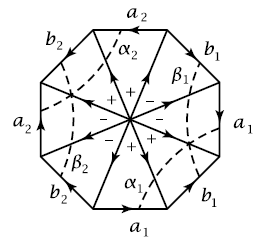
\includegraphics[scale=0.7]{cup}
\caption{Ejemplo del 2-toro.}
\end{figure}

Damos estructura de CW-complejo para calcular cuánto valen estas funciones sobre las células. La orientación de los 2-símplices es antihoraria. Tenemos que encontrar el valor de $\varphi_1$ en los 1-símplices interiores. Tenemos en cuenta que $\delta\varphi_1=0$, es decir, para todo triángulo $t_i$, $\delta\varphi_1(t_1)=\varphi_1(\partial t_i)=\varphi_1([v_0,v_1]+[v_1,v_2]-[v_0,v_2])=\varphi_1([v_0,v_1])+\varphi_1([v_1,v_2])-\varphi_1([v_0,v_2])=0$. Sobre el triángulo que contiene a $a_1$, la arista que está bien orientada valdrá 0 y la que no 1. En el de la derecha obtenemos que el segmento que queda libre debe valer 1 y así el siguiente triángulo,q ue de nuevo contiene a $a_1$ pero está orientado al contrario, está bien evaluado. COMPROBAR QUE DOS ELECCIONES DE VALORES DE PHI SON EN REALIDAD DOS REPRESENTANTES DE ALPHA O MÚLTIPLOS

En la figura anterior se trazan curvas que unen un generador consigo mismo y en cada corte con un 1-símplice se da el valor 1 o $-1$ según la orientación. Esta interpretación cobrará más sentido con la dualidad de Poincaré.

Dada una variedad compacta $M=|K|$, $H^*(M)=H^*(K)=H^*((C_*(K),\delta^*))$. Podemos definir una aplicación $C_q(K)\to C_{n-q}(K)$ dada por $\sum\sigma_i\mapsto \sum\sigma_i^*$, donde el dual de un símplice se define de la siguiente forma. Recordemos que $sd(K)=\{(b(\sigma_0),\dots, b(\sigma_n)\mid \sigma_0<\cdots<\sigma_n\}$, de modo que definimos $\sigma^*=\{(\sigma_0=\sigma<\sigma_1<\cdots)\mid (b(\sigma_0),b(\sigma_1),\dots)\in sd(K)\}$. En la figura anterior, la curva une el baricentro de $a_1$ consigo mismo mediante símplices pasando por los baricentros de los 2-símplices que contienen a $a_1$.  


En cualquier caso, ahora podemos calcular $[\varphi_1\smile \psi_1]\in H^2(M_g)$. Tenemos que $$\varphi_1\smile\psi_1(t_1)=\varphi_1\smile\psi_1([v_0,v_1,v_2])=\varphi_1([v_0,v_1])\psi_1([v_1,v_2])=\varphi_1([v_0,v_1])\cdot 0=0.$$ Se comprueba análogamente que para $j\neq 2$, $(\varphi_1\smile \psi_1)(t_j)=0$. En cambio $$\varphi_1\smile\psi_1(t_2)=\varphi_1([v_0,v_1])\psi_1([v_1,v_2])=1\cdot 1=1.$$ Este cálculo se puede predecir viendo dónde se cortan las curvas del dibujo.

 Sabemos que $H_2(M_g)\cong\Z$ generado por $w=[t_1+t_2-t_3-t_4+t_5+t_6-t_7-t_8]$ (el signo depende de la orientación de $a_i$ o $b_i$). Por otra parte, $H^2(M_g)\cong \Hom(H_2(M_g),\Z)$ mediante el isomorfismo $[f]=\gamma\mapsto h(\gamma)=w^*$. Por lo que $h(\gamma)(w)=1=w^*(w)=\rho(t_1)+\rho(t_2)+\cdots$. Como justamente $\varphi_1\smile\psi_1(t_1+t_2-t_3+\cdots)=1$, tenemos que $\alpha_1\smile\beta
 _1=[\varphi_1\smile\psi_1]=\gamma$. Se comprueba que $\alpha_i\smile\alpha_j=\beta_i\smile\beta_j=0$ para todo $i,j$ y que $\alpha_i\smile\beta_i=\gamma$ (por conmutativiad, $\beta_i\smile\alpha_i=-\gamma$). 


\end{ej}
\begin{ej}
El caso de una superficie no orientable $N_g$ es trivial porque su homología con coeficientes en $\Z$ es nula en dimensión mayor o igual que 2. Aplicando coeficientes universales nos queda 
$$H^q(N_g,\Z)=\begin{cases}
0 & q\geq 2\\
\Z\underbrace{\times\cdots\times}_{q-1}\Z & q=1\\
\Z & q=0
\end{cases}$$

Sin embargo, 

$$H_q(N_g,\Z_2)=\begin{cases}
\Z_2 & q=2\\
(\Z_2)^g & q=1\\
\Z_2 & q=0
\end{cases}$$
y es nula en otro caso. Esto nos da los mismos grupos de cohomología por el teorema de coeficientes universales. Con el isomorfismo $H^1(N_g;\Z_2)\cong \Hom(H_1(N_g);\Z_2)$ hacemos el ejemplo de $N_4$. En este caso además no hay signos. 

\begin{figure}[h!]
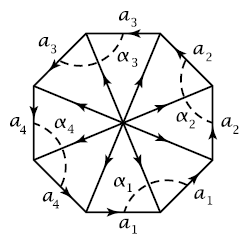
\includegraphics[scale=0.7]{3-8}
\end{figure}

Igual que en el ejemplo anterior el isomorfismo funciona como $\alpha_i=[\varphi_i]\mapsto h(\alpha_i)=[\alpha_i]^*\in H_1(N_g)\to\Z_2$. Es fácil comprobar que $\alpha_i\smile\alpha_j=[\varphi_i\smile\varphi_j]=0$ cuando $i\neq j$. 

$$\varphi_1\smile\varphi_1(t_1)=\varphi([v_0,v_1])\varphi_1([v_1,v_2])=0$$
$$\varphi_1\smile\varphi_1(t_2)=1$$
y en los demás triángulos vale claramente 0. Si denotamos $\gamma$ al generador de $H^2(N_g;\Z_2)$, $h(\gamma)=[\sum t_i]^*$. Tenemos que $h(\alpha_1\smile\alpha_1)([\sum t_i])=1$, luego $\alpha_1\smile\alpha_1=\alpha_1^2=\gamma$. 
\end{ej}

\begin{ej}
Sea $X=B^2\cup_\varphi S^1$ donde $\varphi:\partial B^2\to S^1$ es una aplicación de grado $m$. Viéndo estos espacios como subespacios de $\C$ podemos pensar que es $z\mapsto z^m$. El complejo de cadenas es de la forma $0\to\Z\xrightarrow{m}\Z\xrightarrow{0}\Z\to 0$. Tenemos 

\[
H_q(X;\Z)=\begin{cases}
0 & q\geq 2\\
\Z_m & q=1\\
\Z & q=0
\end{cases}
\]

\[
H^q(X;\Z)=\begin{cases}
0 & q\geq 3\\
\Z_m & q=2\\
0 & q=1\\
\Z & q=0
\end{cases}
\]

De nuevo el cup producto no tiene interés con estos coeficientes, pero con coeficientes en $\Z_m$, la multiplicación por $m$ se vuelve nula y tenemos que 

Hacemos un ejemplo con $m=4$.

\begin{figure}[h!]
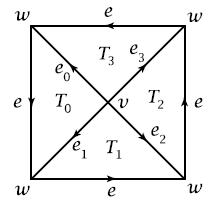
\includegraphics[scale=0.7]{3-9}
\end{figure}

Tenemos del teorema de coeficientes universales que $\Z_m\cong H^1(X;\Z_m)\cong_h\Hom(H_1(X);\Z_m)$ generado por $[\varphi]$. Necesariamente $h([\varphi])=[e]^*$. Como $\varphi$ es un cociclo, $0=\delta\varepsilon(t_i)=\varphi(\partial t_i)=\varphi(e_i+e-e_{i+1})=\varphi(e_i)+1-\varphi(e_{i+1})$ con $i\in\Z_m$. Por tanto, para todo $i$, $\varphi(e_{i+1})=\varphi(e_i)+1$. Pongamos $\varphi(e_i)=i\mod n$. Calculamos ahora $[\varphi]\smile[\psi]=[\varphi\smile\psi]$. 

$$
(\varphi\smile\varphi)(t_i)=\varphi(e_i)\varphi(e)=i\mod n
$$

Vamos a probar con una demostración parecida a la del teorema de coeficientes universales que $h:H^2(X;\Z_m)\to \Hom(H_2(X;\Z_m),\Z_m)$ es isomorfismo. En la demostración del teorema de coeficientes universales usábamos que $B_n$ era libre para que las sucesiones exactas fueran escindibles. En este caso particular vamos a ver que la sucesión exacta es escindible, por lo que se podría continuar a partir de ahí. Tenemos $C_*(X;\Z_m)=\{0\to \Z_m\xrightarrow{0} \Z_m\xrightarrow{0}\Z_m\to 0\}$ (estos $\Z_m$ provienen en realdiad de hacer $\Z\otimes\Z_m$ al el complejo $C_*(X)$). Así que las sucesiones exactas cortas $0\to\Z_{n+1}\to C_{n+1}\to B_n\to 0$ son de la forma $0\to\Z_m\to Z_m\to 0\to 0$. Dualizando obtenemos la misma sucesión pero con las flechas en sentido contrario. La inclusión $B_n\hookrightarrow Z_n$ inducía una aplicación $i^*$ enlazando las sucesiones exactas cortas. Obtendríamos siguiendo la prueba del teorema de coeficientes universales
\[
\ker i^*_2\leftarrow H^2(X;\Z_m)\leftarrow\coker i_1^*=0
\]
Tenemos entonces un isomorfismo $H^2(X;\Z_m)\ker i^*_2=\Hom(H_2(X;\Z_m),\Z_m)$ dado por la aplicación $h$. Entonces buscamos $\zeta=[\psi]\in H^2(X;\Z_m)\mapsto h(\zeta)[\sum_{i=0}^3t_i]=\sum_{i=0}^4\psi(t_i)=1$. Tomamos $\psi:C_2(X)\to\Z_m$ dado por $t_i\mapsto\psi(t_i)=\delta_{1i}$, que es un generador. 

\[
h([\varphi]\smile[\varphi])([\sum_{i=0}^3t_i])=\sum_{i=0}^3\varphi(e_i)\varphi(e)=\sum_{i=0}^3i\mod 4=0+1+2+3=\frac{m(m-1)}{2}\mod m
\]
Si $m=2k$, entonces este producto es congruente con $k\mod m$. Si $m$ es impar, $m-1$ es impar y el producto sería congruente con $mk\equiv 0\mod m$. Así que 
\[
[\varphi]\smile[\varphi]=\begin{cases}
0 & m\text{ impar}\\
k\zeta & m\text{ par}
\end{cases}
\]
En nuestro caso tenemos $m$ par. 
\end{ej}






El cup producto también se restringe a las cadenas relativas $C^*(X,A)\subseteq C^*(X)$ para un subespacio $A\subseteq X$. Si $\varphi\in C^*(X,A)$ y $\sigma$ es un símplice singular cuya imagen está contenida en $A$, su restricción también está contenida en $A$, luego $\varphi(\sigma|)=0$, con lo que $(\varphi\smile\psi)(\sigma)=0$, con lo que $\varphi\smile\psi\in C^*(X,A)$. Nótese que no hemos necesitado que $\psi$ sea una cocadena relativa, luego tenemos cup-productos tanto $C^*(X,A)\times C^*(X)\to C^*(X,A)$ como $C^*(X,A)\times C^*(X,A)\to C^*(X,A)$. La misma prueba que en el caso no relativo sirve para inducir un cup producto en homología. Además tenemos inclusiones $C^*(X,A)\times C^*(X,A)\hookrightarrow C^*(X,A)\times C^*(X)\hookrightarrow C^*(X)\times C^*(X)$.  Así que los cup productos son compatibles con la sucesión exacta larga de cohomología a través del diagrama conmutativo
\[
\begin{tikzcd}
H^p(X,A;R)\times H^q(X;R)\arrow[r]\arrow[d, "j\times Id"] & H^{p+q}(X,A;R)\arrow[d, "j"]\\
H^p(X;R)\times H^q(X;R)\arrow[r] & H^{p+q}(X;R)
\end{tikzcd}
\]
Si llamamos $j$ a la aplicación $H^n(X,A;R)\to H^n(X;R)$ en la sucesión exacta larga de cohomología relativa y tomamos un par $([\varphi],[\psi])\in H^p(X,A;R)\times H^q(X;R)$ tenemos que $j([\varphi]\smile [\psi])=j([\varphi])\smile[\psi]$. Análogamente podríamos poner la cohomología relativa en la izquierda en lugar de en la derecha. 

\begin{lemma}
Sea $f:X\to Y$, $\varphi,\psi\in C^*(Y)$. Entonces la aplicación $f^\sharp:C^*(Y)\to C^*(X)$ verifica $f^\sharp(\varphi\smile\psi)=f^\sharp(\varphi)\smile f^\sharp(\psi)\in C^{p+q}(X;R)$ (es un homomorfismo de anillos).
\end{lemma}
\begin{proof}
Sea $\sigma:\Delta^{p+q}\to X$. Entonces
\[
f^\sharp(\varphi\smile\psi)(\sigma)=(\varphi\smile\psi)(f\sigma)=\varphi(f\sigma|_{[v_0,\dots, v_p]})\psi(f\sigma|_{[v_p,\dots, v_{p+q}]})=\]
\[
=f^\sharp(\varphi)(\sigma_{[v_0,\dots, v_p]}) f^\sharp(\psi)(\sigma_{[v_p,\dots, v_{p+q}]})=(f^\sharp(\varphi)\smile f^\sharp(\psi))(\sigma)
\]
Como esta igualdad se verifica para todos los elementos de la base, se verifica para todo el espacio. 
\end{proof}
Entonces $f^*:H(Y)\to H^*(X)$ preserva el producto cup y análogamente con el complejo relativo. En particular esto se verifica para $i^*$ en la sucesión exacta larga de cohomología de un par. Nos falta ver la relación con el homomorfismo de conexión de la sucesión exacta larga. 

BUSCAR RELACIÓN. EL PRODUCTO DE UN ELEMENTO DE $H^{n+1}(X,A;R)$ CON UNO DE $H^n(X;R)$ (ALOMEJOR AQUÍ HAY ALGO C \url{http://www.hiroleetanaka.com/pdfs/231a-hmwk12.pdf})

Sean $A,B\subseteq X$ abiertos. Veamos que existe también un cup producto $H^*(X;A;R)\times H^*(X,B;R)\to H^*(X,A\cup B;R)$. Desgraciadamente, el producto de una cocadena en $C^*(X,A;R)$ con una de $C^*(X,B;R)$ no está en general en $C^*(X,A\cup B;R)$. Recordemos la equivalencia homotópica $C_*(A+B)\hookrightarrow C_*(A\cup B)$. Aplicando el functor $\Hom(-,R)$ obtenemos la equivalencia $C^*(A\cup B;R)\twoheadrightarrow C^*(A+B;R)$. Además tenemos el diagrama conmutativo
\[
\begin{tikzcd}
C^*(A+B;R) & C^*(A\cup B;R)\arrow[l, twoheadrightarrow]\\
C^*(X;R)\arrow[u, twoheadrightarrow]\arrow[r, equals] & C^*(X;R)\arrow[u, twoheadrightarrow]\\
C^*(X,A+B;R)\arrow[u, hookrightarrow] & C^*(X,A\cup B;R)\arrow[l, hookrightarrow]\arrow[u, hookrightarrow]
\end{tikzcd}
\]
El término de abajo a la izquierda no es más que notación para el núcleo de la aplicación superior. Aplicando el lema de los cinco al morfismo entre sucesiones exactas largas de cohomología de estas sucesiones exactas cortas, encontramos que la aplicación de abajo induce isomorfismo en cohomología. 

Con esto tenemos un cup producto $C^*(X,A;R)\times C^*(X,B;R)\to C^*(X,A+B;R)$, que induce un cup producto en cohomología, que por lo anterior nos da el cup producto que queríamos. 

\begin{teorema}
Sea $X$ un espacio topológico y $\alpha,\beta\in H^*(X)$ con $|\alpha|=p$ y $|\beta|=q$ (los grados en cohomología). Entonces $\alpha\smile \beta=(-1)^{pq}\beta\smile\alpha$. 
\end{teorema}
\begin{dem}
Sean $\alpha=[\varphi]$ y $\beta=[\psi]$. Nótese que a nivel de cocadenas la conmutatividad no se verifica en general porque cada restricción se hace sobre distintas caras del símplice singular. Vamos a ver que podemos cambiar el orden de los vértices sin que esto afecte a la cohomología. Denotamos $\Delta^n:[v_0,\dots, v_n]$. Dado $\sigma:\Delta^n\to X$ definimos $\overline{\sigma}:\Delta^n\to\Delta^n\to X$, donde la primera aplicación es un isomorfismo lineal $v_i=v_{n-i}$. El signo de esta permutación de los índices es $(-1)^{\sum_{i=0}^ni}=(-1)^{\frac{n(n+1)}{2}}=\varphi_n$. Definimos $\rho:C_*(X)\to C_*(X)$ como $\sigma\mapsto\varepsilon_n\overline{\sigma}$. Vamos a ver que esto es un morfismo de complejos de cadenas. 

Tenemos que $d(\sigma)=\sum_{i=0}^n(-1)^i\sigma|_{[v_0,\dots, \hat{v}_i,\dots, v_n]}$. Entonces 
\[
\rho d(\sigma)=\varepsilon_{n-1}\sum_{i=0}^n(-1)^i\overline{\sigma|_{[v_0,\dots, \hat{v}_i,\dots, v_n]}}.
\]
Por otro lado
\[
d\rho(\sigma)=\varepsilon_nd(\overline{\sigma})=\varepsilon_n\sum_{i=0}^n(-1)^i\overline{\sigma}|_{[v_0,\dots, \hat{v}_i,\dots, v_n]}
\]
La diferencia entre restringir antes o después de aplciarle el isomorfismo lineal es que en lugar de omitir $i$ se omite $n-i$, luego bata comprobar que el signo en cada uno es el mismo. Como $\varepsilon_{n-1}(-1)^i=\varepsilon_n(-1)^{n-i}=\varepsilon_n(-1)^n(-1)^i$, basta comprobar que $\varepsilon_{n-1}=\varepsilon_n(-1)^n$. Efectivamente, $\varepsilon_n=(-1)^{\sum_{i=0}^{n-1}i}(-1)^n=\varepsilon_{n-1}(-1)^n=\varepsilon_n$. 

Veamos ahora que $\rho\simeq Id$. Sea $I=[0,1]$ y consideremos $\Delta^n\times I$. Identificamos $\Delta^n\times\{0\}=\Delta^n$ y a los vértices de $\Delta^n\times\{0\}$ los denotamos $w_0,\dots, w_n$. Sabemos que $\Delta^n\times I$ es un complejo simplicial de dimension $n+1$ con caras de la forma $[v_0,\dots, v_i,w_i,\dots, w_n]$ para $i=0,\dots, n$. Denotamos $\pi:\Delta^n\times I\to \Delta^n$. Vamos a definir una homotopía $P:C_n(X)\to C_{n+1}(X)$ que nos de $dP+Pd=\rho-Id$ mediante $P(\sigma)=\sum_{i=0}^n(-1)^i\varepsilon_{n-i}\sigma\pi|_{[v_0,\dots, v_i,w_n,\dots,w_i]}$. Ahora
\[
dP(\sigma)=\sum_{i=0}^n(-1)^i\varepsilon_{n-i}\left[\sum_{j=0}^i(-1)^j\sigma\pi|_{[v_0,\dots,\hat{v}_j,\dots,  v_i,w_n,\dots,w_i]}+\sum_{j=i}^n(-1)^{n-j+i+1}\sigma\pi|_{[v_0,\dots, v_i,w_n,\dots,\hat{w}_j,\dots, w_i]}\right]
\]
Los términos $i=j$ en estas sumas dan
\[
\varepsilon_n\sigma\pi|_{[v_0,\dots,v_n]}+\sum_{i=1}^n\varepsilon_{n-i}\sigma\pi|_{[v_0,\dots,v_{i-1},w_n,\dots, w_i]}+\sum_{i=1}^{n-1}(-1)^{n+i+1}\varepsilon_{n-i}\sigma\pi|_{[v_0,\dots, v_i,w_n,\dots, w_{i+1}]}-[v_0,\dots, v_n]
\]
En esta expresión los dos sumatorios se cancelan ya que al reemplazar $i$ por $i-1$ en el segundo sumatorio produce un nuevo signo $(-1)^{n+i}\varepsilon_{n-i+1}=-\varepsilon_{n-i}$. Los otros dos términos representan $\rho(\sigma)-\sigma$. Así que para demostrar que $dP+Pd=\rho-Id$ falta mostrar que la formula para $dP$ anterior da $-Pd$ para $i\neq j$. Calculamos entonces
\[
Pd(\sigma)=\sum_{i<j}(-1)^j\varepsilon_{n-i-1}\sigma\pi|_{[v_0,\dots, v_j,w_n,\dots,\hat{w}_j,\dots,w_i]}+\sum_{j>i}(-1)^{i-1}\varepsilon_{n-i}\sigma\pi|_{[v_0,\dots, \dots,\hat{v}_j,v_j,w_n,\dots,w_i]}
\]
Como $\varepsilon_{n-i}=(-1)^{n-i}\varepsilon_{n-i-1}$, esto finaliza la comprobación.


Aplicando $\Hom(-,R)$, $\rho$ induce $\rho^*$ en las cocadenas que también es homotópico a la identidad. Entonces $$\rho^*(\varphi\smile\psi)(\sigma)=(\varphi\smile\psi)(\rho(\sigma))=(\varphi\smile\psi)(\varepsilon_{p+q}\overline{\sigma})=\varepsilon_{p+q}\varphi(\overline{\sigma}|_{[v_0, v_p]})\psi(\overline{\sigma}|_{[v_p,v_{p+q}]}.$$ 
Por otra parte, 

$$
(\rho^*(\psi)\smile\rho^*(\varphi))(\sigma)=\rho^*(\psi)(\sigma|_{[v_0,\dots, v_q]})\rho^*(\varphi)(\sigma|_{[v_0,\dots,v_{p+q}]})=\varepsilon_q\psi(\overline{\sigma|_{[v_0,\dots, v_q]}})\varphi(\overline{\sigma|_{[v_q, \dots,v_{p+q}]}})
$$

Como $\rho^*\simeq Id$, $\alpha=[\rho^*(\varphi)]$ y $\beta=[\rho^*(\psi)]$, luego $\alpha\cup\beta=[\rho^*(\varphi\smile\psi)]$, y como $\varepsilon_{p+q}=\varepsilon_p\varepsilon_q(-1)^{pq}$, se tiene el resultado. 
\end{dem}

\section{Anillo de Cohomología}
Como hemos visto en la sección anterior, el producto cup es asociativo y distributivo, por lo que podemos dotar de estructura de anillo a $H^*(X;R)=\oplus_{i\geq 0}H^i(X;R)$, donde los elementos de este anillo son sumas finitas $\sum_i\alpha_i$ con $\alpha_i\in H^i(X;R)$. El producto de dos tales sumas está definido como $(\sum_i\alpha_i)(\sum_j\beta_j)=\sum_{i,j}\alpha_i\smile\beta_j$. Esto convierte a $H^*(X;R)$ es un anillo, con unidad si $R$ tiene unidad (el elemento unidad será el generador de $H_0(X;R)$ que envía todo símplice singular al $1\in R$). Tomando en cuenta la multiplicación por escalares de $R$ en cuenta, estos anillos pueden ser vistos también como $R$-álgebras. 

El anillo de cohomología se considera siempre como anillo gradudado. Esto es, un anillo $A=\oplus_{k\geq 0}A_k$ donde los $A_k$ son grupos aditivos y e $A_k A_l\subseteq A_{k+l}$. Si $\alpha\in A_k$ escribiremos $|\alpha|=k$ y diremos que tiene \emph{grado} $k$. Cuando además se verifica $ab=(-1)^{|a||b|}ba$ diremos que el anillo es conmutativo (grambién graduado-conmutativo, skew-conmutativo o anticonmutativo).  

\begin{ej}
Anillos de polinomios $R[\alpha]$ y $R[\alpha]/\gene{\alpha^n}$. 
\end{ej}

\begin{ej}
Álgebras exteriores $\land_R[\alpha_1,\dots,\alpha_n]$. Esto es el $R$-módulo libre con base el producto finito (ordenado) $\alpha_{i_1}\land\cdots\land\alpha_{i_k}$, $i_1<\cdots<i_k$ con producto asociativo y distributivo verificando $\alpha_i\land\alpha_j=-\alpha_j\land\alpha_i$. Un ejemplo de este tipo de anillo graduado en cohomología es $H^*(T;\Z)=H^*(S^1\times S^1;\Z)=\bigwedge_\Z[\alpha,\beta]$ por el ejemplo de superficie orientable. En general, para  $T^n$ sale un álgebra exterior en $2n$ generadores, como se prueba en el ejemplo 3.16 de Hatcher.   
\end{ej}

\begin{ej}
Anillos producto. El isomorfismo $H^*(\coprod_\alpha X_\alpha)\cong \prod_\alpha H^*(X_\alpha;R)$ inducido por las inclusiones $i_\alpha:X_\alpha\to X$ es un isomorfismo de anillos pues cada $i_\alpha^*$ lo es. El isomorfismo de anillos de productos viene de la propiedad universal del producto directo, usando las proyecciones $\pi_\alpha:\prod_\alpha H^*(X_\alpha;R)\to H^*(X_\alpha;R)$ y a $H^*(\coprod X_\alpha;R)$ va por otro lado la $(i_\alpha)^*$, además $\{i_\alpha^*\}([\varphi\smile\psi])=\{i^*_\alpha(\varphi)\smile i_\alpha^*(\psi)\}=\{i^*_\alpha(\varphi\smile\psi)\}$ (esta es la aplicación dibujada con línea discontinua en el diagrama).

\[
\begin{tikzcd}
\prod_\alpha H^*( X_\alpha;R)\arrow[r, "\pi_\alpha"] & H^*(X_\alpha;R)\\
H^*(\coprod_\alpha X_\alpha)\arrow[ur, "(i_\alpha)^*"']\arrow[u, dashed]
\end{tikzcd}
\]

 Similarmente $\widetilde{H}^*(\bigvee_\alpha X_\alpha;R)\cong\prod_\alpha\widetilde{H}^*(X_\alpha;R)$, suponiendo que $x_\alpha\in X_\alpha$ son retractos de deformación de un entorno suyo para poder aplicar escisión y garantizar el isomorfismo. Esta estructura extra sirve para distinguir $S^2\vee S^4$ de $\C P^2$, que es el resultado de pegar una 4-célula a $S^2$ mediante $f:S^3\to S^2$. Tenemos que $\widetilde{H}^*(S^2\vee S^4;\Z)\cong \widetilde{H}^*(S^2)\oplus \widetilde{H}^*(S^4)$, de modo que visto como anillo, el producto de los generadores de $H^2(S^2)$ es nulo al estar el resultado en $H^4(S^2)=0$. Sin embargo, $H^*(\C P^2;\Z)=\Z[\alpha]/\gene{\alpha^3}$ con $|\alpha|=2$ como se probará más adelante, por lo que producto del generador de grado 2 consigo mismo de $H^2(\C P^2;\Z)$ no es nulo.
\end{ej}

\subsection{Fórmula de Künneth}
\begin{defi}
El \emph{producto cross} $H^*(X;R)\times H^*(Y;R)\to H^*(X\times Y;R)$ está definido como $(a,b)\mapsto a\times b=p_1^*(a)\smile p_2^*(b)$, donde $p_i$ son las proyecciones $X\times Y\to X,Y$. 
\end{defi}

Como el cup producto es distributivo, el producto cross es bilineal (lineal en cada coordenada por separado), pero esto no implica que sea un homomorfismo, mucho menos un isomorfismo. Para conseguir que sea un homomorfismo reemplazamos $H^*(X;R)\times H^*(Y;R)$ por el producto tensorial $H^*(X;R)\otimes_R H^*(Y;R)$. Repasemos la definición del producto tensorial y sus propiedades básicas. Dados dos grupos abelianos $A$ y $B$, $A\otimes B$ es el grupo abeliano con elementos $a\otimes b$ verificando:
\begin{enumerate}
\item $(a+a')\otimes b=a\otimes b+a'\otimes b$.
\item $a\otimes (b+b')=a\otimes b+a\otimes b'$.
\item $0\otimes 0=a\otimes 0=0\otimes b$.
\item $-(a\otimes b)=-a\otimes b=a\otimes -b$
\end{enumerate} 

Obsérvese que $A\otimes B$ no es más que un cociente de $A\times B$ por la relación generada por las propiedades anteriores. Se verifican las propiedades elementales siguientes:
\begin{enumerate}
\item $A\otimes B\cong B\otimes A$.
\item $(\oplus_i A_i)\otimes B\cong \oplus_i(A_i\otimes B)$.
\item $(A\otimes B)\otimes C\cong A\otimes (B\otimes C)$.
\item $\Z\otimes A\cong A$.
\item $\Z_n\otimes A\cong A/nA$. 
\item Dados homomorfismos $f:A\to A'$ y $g:B\to B'$, se induce un homomorfismo $f\otimes g:A\otimes B\to B\otimes B'$ dado por $(f\otimes g)(a\otimes b)=f(a)\otimes g(b)$. 
\item Toda aplicación bilineal $\varphi:A\times B\to C$ induce un homomorfismo $A\otimes B\to C$ enviando $a\otimes b$ a $\varphi(a,b)$. 
\end{enumerate}

Para generalizar el producto tensorial a la categoría de $R$-módulos con $R$ conmutativo definimos $A\otimes_R B$ como el cociente de $A\otimes B$ obtenido al imponer la relación $ra\otimes b=a\otimes rb$. Si $R$ no es conmutativo, pedimos que $A$ sea $R$-módulo por la derecha y $B$ sea $R$-módulo por la izquierda e imponemos la relación $ar\otimes b=a\otimes rb$. En este caso $A\otimes_R B$ es solo un grupo abeliano. Es sencillo comprobar que cuando $R=\Z_m$ o $\Q$, $A\otimes_R B=A\otimes B$, pero en general no es cierto. 

Las propiedades 1-3, 6 y 7 siguen siendo válidas para el caso de $R$-módulos. La 4 tiene un generalización sencilla $R\otimes_R A\cong A$ mediante $r\otimes a\mapsto ra$. Por 7 el producto cross induce un homomorfismo de $R$-módulos que también llamaremos producto cross
\[
H^*(X;R)\otimes_R H^*(Y;R)\to H^*(X\times Y;R),\ a\otimes b\mapsto a\times b
\]


Este producto se convierte en un homomorfismo de anillos si definimos el producto como $(a\otimes b)(c\otimes d)=(-1)^{|b||c|}(ac)\otimes (bd)$, donde $|x|$ denota el grado de $x$. Efectivamente, denotando por $\mu$ al producto cross

\begin{align*}
\mu((a\otimes b)(c\otimes d))=&\mu((-1)^{|b||c|}(ac)\otimes (bd))=(-1)^{|b||c|}(a\smile c)\times (b\smile d)\\
=&(-1)^{|b||c|}(p_1^*(a\smile c)\smile p_2^*(b\smile d))\\
=&(-1)^{|b||c|}(p_1^*(a)\smile p_1^*(c)\smile p_2^*(b)\smile p_2^*(d))\\
=&p_1^*(a)\smile p_2^*(b)\smile p_1^*(c)\smile p_2^*(d))=(a\times b)\smile (c\times d)\\
=&\mu(a\otimes b)\smile \mu (c\otimes d)=\mu(a\otimes b)\mu(c\otimes d)
\end{align*}

\begin{teorema}[Fórmula de Künneth]\label{tensor}
El producto cross $\mu:H^*(X;R)\otimes_R H^*(Y;R)\to H^*(X\times Y;R)$ es un isomorfismo de anillos si $X$ e $Y$ son CW-complejos y $H^k(Y;R)$ es finitamente generado para todo $k$.
\end{teorema}

\begin{nota}
La hipótesis de ser CW-complejos no es necesaria (ver 3.B y 3.E de Hatcher).
\end{nota}

%\frown -> cap product

AÑADIR A LA BIBLIOGRAFÍA SPANIER, DONDE VIENE LA PRUEBA QUE UTILIZA MÁS TEORÍA.

BUSCAR FUNCTOR TOR EN HATCHER 3.A

La idea de la prueba será considerar, para un CW complejo $Y$, los functores de pares de CW
\begin{gather*}
h^n(X,A)=\bigoplus_i(H^i(X,A;R)\otimes_R H^{n-1}(Y;R))\\
k^n(X,A)=H^n(X\times Y,A\times Y;R)
\end{gather*}
El producto cross, o su versión relativa (la veremos más adelante), define una aplicación $\mu: h^n(X,A)\to k^n(X,A)$ que nos gustaría probar que es isomorfismo cuando $X$ es un CW complejo y $A=\emptyset$. Probaremos:
\begin{enumerate}
\item $h^*$ y $k^*$ son teorías de cohomología en la categoría de CW complejos.
\item $\mu$ es una transformación natural: conmuta con las aplicaciones inducidas y con el operador coborde. 
\end{enumerate}

Es obvio que $\mu:h^n(*,\emptyset)\to k^n(*,\emptyset)$ es un isomorfismo ya que es simplemente la multiplicación por escalar $R\otimes_R H^n(Y;R)\to H^n(Y;R)$. La siguiente proposición implicará el teorema:

\begin{prop}
Si una transformación natural entre teorías de cohomología (no reducida) sobre la categoría de pares CW es un isomorfismo para el par $(*,\emptyset)$, entonces es un isomorfismo para todos los pares de CW.
\end{prop}
\begin{dem}
Si $\mu$ es una transformación natural entre las cohomologías $h^*$ y $k^*$ entonces
\[
\begin{tikzcd}
\cdots \arrow[r] & h^{n-1}(X) \arrow[r] \arrow[d, "\mu"] & h^{n-1}(A) \arrow[r] \arrow[d, "\mu"] & {h^{n}(X,A)} \arrow[r] \arrow[d, "\mu"] & h^{n}(X) \arrow[d, "\mu"] \arrow[r] & h^{n}(A) \arrow[r] \arrow[d, "\mu"] & \cdots \\
\cdots \arrow[r] & k^{n-1}(X) \arrow[r] & k^{n-1}(A) \arrow[r] & {k^{n}(X,A)} \arrow[r] & k^{n}(X) \arrow[r] & k^{n}(A) \arrow[r] & \cdots
\end{tikzcd}
\]
conmuta. Por lo que, usando el lema de los cinco, basta comprobar el isomorfismo de $\mu$ en el caso absoluto con $A=\emptyset$ para tenerlo en todas las parejas. Probamos primero el caso finito-dimensional por inducción en la dimensión de $X$. Si $\dim(X)=0$, entonces $X=\coprod_{i=1}^r\{x_i\}$ y por tanto $h^n(X)=\prod_{i=1}^rh^n(x_i)$ y $k^n(X)=\prod_{i=1}^r k^n(x_i)$, de modo que por hipótesis son isomorfas. 

Supongámoslo ahora cierto para dimensiones a lo sumo $n-1$ y consideramos el par $(X^n,X^{n-1})$, para el cual tenemos el diagrama conmutativo
\[
\begin{tikzcd}[column sep=18]
\cdots \arrow[r] & h^{q-1}(X^n) \arrow[r] \arrow[d, "\mu"] & h^{q-1}(X^{n-1}) \arrow[r] \arrow[d, "\mu"] & {h^{q}(X^n,X^{n-1})} \arrow[r] \arrow[d, "\mu"] & h^{q}(X^n) \arrow[d, "\mu"] \arrow[r] & h^{n}(X^{n-1}) \arrow[r] \arrow[d, "\mu"] & \cdots \\
\cdots \arrow[r] & k^{q-1}(X^n) \arrow[r] & k^{q-1}(X^{n-1}) \arrow[r] & {k^{q}(X^n,X^{n-1})} \arrow[r] & k^{q}(X^n) \arrow[r] & k^{n}(X^{n-1}) \arrow[r] & \cdots
\end{tikzcd}
\]
que por el lema de los cinco, nos indica que basta comprobar el resultado para parejas $(X^n,X^{n-1})$ para tenerlo para $X^n$.

Sea $\Phi:\coprod_{\alpha}(D_\alpha^n,S_\alpha^{n-1})\to (X^n,X^{n-1})$ la colección de aplicaciones características de las $n$-células de $X$. Por escisión obtenemos que $\Phi^*$ induce isomorfismos para $h^*$ y $k^*$
\[
\begin{tikzcd}
{h^*(X^n,X^{n-1})} \arrow[r, "\Phi^*"] \arrow[d, "\mu"] & {\prod_\alpha h^*(D_\alpha^n,S_\alpha^{n-1})} \arrow[d, "\prod_\alpha\mu_\alpha"] \\
{k^*(X^n,X^{n-1})} \arrow[r, "\Phi^*"] & {\prod_\alpha k^*(D_\alpha^n,S_\alpha^{n-1})}
\end{tikzcd}
\]
Usando el axioma de uniión disjunta y la naturalidad de $\mu$, basta probar que $\mu$ induce isomorfismo para $(D^n,S^{n-1})$. Como $\mu$ es isomorfismo para puntos, lo es para $D^n$ por homotopía y también lo es para $S^{n-1}$ por inducción sobre la dimensión. Por el lema de los 5 aplicado a 
\[
\begin{tikzcd}[column sep=18]
\cdots \arrow[r] & h^{q-1}(D^n) \arrow[r] \arrow[d, "\mu"] & h^{q-1}(S^{n-1}) \arrow[r] \arrow[d, "\mu"] & {h^{q}(D^n,S^{n-1})} \arrow[r] \arrow[d, "\mu"] & h^{q}(D^n) \arrow[d, "\mu"] \arrow[r] & h^{n}(S^{n-1}) \arrow[r] \arrow[d, "\mu"] & \cdots \\
\cdots \arrow[r] & k^{q-1}(D^n) \arrow[r] & k^{q-1}(S^{n-1}) \arrow[r] & {k^{q}(D^n,S^{n-1})} \arrow[r] & k^{q}(D^n) \arrow[r] & k^{n}(S^{n-1}) \arrow[r] & \cdots
\end{tikzcd}
\]
se deduce que el isomorfismo es cierto para $(D^n,S^{n-1})$. 

El caso infinito-dimensional se sigue del caso anterior, pues de los axiomas se deduce que las inclusiones $X^n\hookrightarrow X$ inducen isomorfismo para $n$ suficientemente grande con respecto a $q$ en $h^q(X)\to h^q(X^n)$ y $k^q(X)\to k^q(X^n)$.
\end{dem}

\begin{dem}[del teorema \ref{tensor}]
Falta ver que $h^*$ y $k^*$ son teorías de cohomología y que $\mu$ es una transformación natural entre ellas. 

\begin{enumerate}
\item Invariancia homotópica: Si $f\simeq g$, entonces$f^*=g^*$. Esto es obvio para $h^*$ y para $k^*$. 
\item Excisión: Si $X=A\cup B$ es unión de subcomplejos, entonces claramente $h^*(X,A)=h^*(A,A\cap B)$. Para $k^*$ también es claro porque $(A\cup B)\times Y=(A\times Y)\cup (B\times Y)$ y $(A\cap B)\times Y=(A\times Y)\cap (B\times Y)$. 
\item Sucesión exacta larga de una pareja: es trivial para $k^*$. Para $h^*$, como $H^{n-i}(Y;R)$ es libre y finitamente generado PREGUNTAR POR ESTO, entonces $-\otimes H^{n-i}(Y;R)$ preserva la exactitud de 
\[
\cdots\to H^i(X,A)\to H^i(X)\to H^i(A)\to H^{i+1}(X,A)\to\cdots
\]
Variando $i$ y tomando la suma directa en $i=0,\dots, n$ de las sucesiones exactas previas obtenemos el resultado para $h^*$. 
\[
\begin{tikzcd}
\vdots \arrow[d] & \vdots \arrow[d] \\
{H^i(X,A)\otimes H^{n-i}(Y;R) } \arrow[d] & {H^{i+1}(X,A)\otimes H^{n-i-1}(Y;R)} \arrow[d] \\
H^i(X)\otimes H^{n-i}(Y;R) \arrow[d] & H^{i+1}(X)\otimes H^{n-i-1}(Y;R) \arrow[d] \\
H^i(A)\otimes H^{n-i}(Y;R) \arrow[d] & H^{i+1}(A)\otimes H^{n-i-1}(Y;R) \arrow[d] \\
{H^{i+1}(X,A)\otimes H^{n-i}(Y;R)} \arrow[d] & {H^{i+2}(X,A)\otimes H^{n-i-2}(Y;R)} \arrow[d] \\
\vdots & \vdots
\end{tikzcd}
\]
\item Uniones disjuntas: de nuevo es obvio para $k^*$. Para $h^*$ usamos el isomorfismo canónico $(\prod_\alpha M_\alpha)\otimes_R N\cong \prod_\alpha (M_\alpha\otimes_R N)$ para $N$ libre y finitamente generado. Como $N=\prod R_\beta$ es producto finito (o suma directa) de copias $R_\beta$, entonces cada $M\otimes_R N$ es el producto finito de copias $M_{\alpha\beta}=M_\alpha\otimes_R R_\beta$. Entonces, la relación que buscábamos es
\[
\prod_\beta\prod_\alpha M_{\alpha\beta}\cong\prod_\alpha\prod_\beta M_{\alpha\beta}
\]
que es trivialmente cierta. Así, tenemos
\begin{gather*}
h^n\left(\coprod_\alpha(X_\alpha, A_\alpha)\right)=\bigoplus_i\left(H^i\left(\coprod_\alpha(X_\alpha, A_\alpha)\right)\otimes H^{n-i}(Y)\right)=\\
\bigoplus_i\left( \prod_\alpha H^i(X_\alpha,A_\alpha)\otimes H^{n-i}(Y)\right)
\end{gather*}
y por tanto
\begin{gather*}
\prod_\alpha h^n(X_\alpha,A_\alpha)=\prod_\alpha\left(\bigoplus_i H^i(X_\alpha,A_\alpha)\otimes H^{n-i}(Y)\right)=\\
\bigoplus_i\prod_\alpha\left(H^i(X_\alpha,A_\alpha)\otimes H^{n-i}(Y)\right)
\end{gather*}
\end{enumerate}
Ahora tenemos que probar la naturalidad de $\mu$. La naturalidad con respecto a las aplicaciones entre espacios se deduce de la naturalidad del producto cup. La naturalidad respecto al operador borde se sigue de la conmutatividad del siguiente diagrama
\[
\begin{tikzcd}
H^k(A;R)\times H^l(Y;R) \arrow[r, "\delta\times Id"] \arrow[d, "\times"] & H^{k+1}(A;R)\times H^l(Y;R) \arrow[d, "\times"] \\
H^{k+l}(A\times Y;R) \arrow[r, "\delta"] & H^{k+l+1}(A\times Y;R)
\end{tikzcd}
\]
Para comprobarla, empecemos con un elemento del producto arriba a la izquierda, representado por cociclos $\varphi\in C^k(A;R)$ y $\psi\in C^l(Y;R)$. Extendemos $\varphi$ a una cocadena $\overline{\varphi}\in C^k(X;R)$ (por ejemplo con el homomorfismo inducido por la inclusión). Entonces el par $(\varphi,\psi)$ se envía a la derecha a $(\delta\overline{\varphi}, \psi)$ y luego hacia abajo a $p_1^*(\delta\overline{\varphi})\smile p_2^*(\psi)$. Yendo en el otro sentido del cuadrado, $(\varphi,\psi)$ se envía hacia abajo a $p_1^*(\varphi)\smile p_2^*(\psi)$ y luego a la derecha a $\delta(p_1^*(\overline{\varphi})\smile p_2^*(\psi))$, ya que $p_1^*(\overline{\varphi})\smile p_2^*(\psi)$ extiende a $p_1^*(\varphi)\smile p_2^*(\psi)$ sobre $X\times Y$. Finalmente, $\delta(p_1^*(\overline{\varphi})\smile p_2^*(\psi))=p_1^*(\overline{\varphi})\smile p_2^*(\psi)$ ya que $\delta\psi=0$. POR QUÉ ES 0
\end{dem}

La versión relativa del producto cross es
\[
H^*(X,A;R)\otimes_r H^*(Y,B;R)\xrightarrow{\times} H^*(X\times Y,A\times Y\cup X\times B;R)
\]
definido como el el caso absoluto mediante $a\otimes b\mapsto a\times b=p_1^*(a)\smile p_2^*(b)$, donde $p_1^*(a)\in H^*(X\times Y,A\times Y;R)$ y $p_2^*(b)\in H^*(X\times Y,X\times B;R)$. 

\begin{teorema}[Fórmula de Künneth relativa]
Para pares CW, el homomorfismo anterior es isomorfismo de anillos si $H^k(Y;R)$ es libre y finitamente generado como $R$-módulo para todo $k$. 
\end{teorema}
\begin{dem}
El caso $B=\emptyset$ ya has sido probado para la versión absoluta. Con el siguiente diagrama conmutativo reduciremos el caso $B\neq\emptyset$ al de que $B$ sea un punto. 
\[
\begin{tikzcd}
{H^*(X,A)\otimes_R H^*(Y,B) } \arrow[r, "\cong"] \arrow[d, "\times"] & {H^*(X,A)\otimes_R H^*(Y/B,B/B)} \arrow[d, "\times"] \\
{H^*(X\times Y,A\times Y\cup X\times B)} \arrow[r, "\cong"] & {H^*(X\times (Y/B), A\times (Y/B)\cup X\times (B/B))}
\end{tikzcd}
\]
La flecha superior es isomorfismo por escisión y la inferior resulta de que los espacios cociente $(X\times Y)/(A\times Y\cup X\times B)$ y $(X\times (Y/B))/(A\times (Y/B)\cup X\times (B/B))$ son homeomorfos. 

Tomando entonces $B=\{y_0\}\subseteq Y$ tenemos el diagrama conmutativo
\[
\begin{tikzcd}[column sep=20]
{H^*(X,A)\otimes_R H^*(Y,y_0)} \arrow[r] \arrow[dd, "\times"] & {H^*(X,A)\otimes_R H^*(Y)} \arrow[r] \arrow[dd, "\times"] & {H^*(X,A)\otimes_R H^*(y_0)} \arrow[d, "\times"] \\
 &  & {H^*(X\times y_0,A\times y_0)}  \\
{H^*(X\times Y,X\times y_0\cup A\times Y) } \arrow[r] & {H^*(X\times A,A\times Y)} \arrow[ru] \arrow[r] & {H^*(X\times y_0\cup A\times Y,A\times Y)}\arrow[u, "\cong"]
\end{tikzcd}
\]
La fila superior es una sucesión exacta corta escindible porque $y_0$ es retracto de $Y$ (con escición dada por el retracto). El morfismo vertical inferior en la columna derecha es isomorfismo usando escisión y el homeomorfismo de los cocientes. Así la fila inferior también es sucesión exacta corta escindible porque $(X\times \{y_0\},A\times\{y_0\})$ es retracto de $(X\times Y,A\times Y)$. Los morfismos verticales del centro y la derecha son isomorfismos por el caso $B=\emptyset$. Así que por el lema de los cinco obtenemos el resultado para $B=\{y_0\}$. 
\end{dem}

El producto cross relativo da lugar a un producto cross reducido 
\[
\widetilde{H}^*(X;R)\otimes_R\widetilde{H}^*(Y;R)\to \widetilde{H}^*(X\wedge Y;R)
\]
recordamos que $X\wedge Y=(X\times Y)/(X\times\{x_0\}\cup \{x_0\}\times Y)$. Este producto es isomorfismo si $\widetilde{H}^*(X;R)$ o $\widetilde{H}^*(Y;R)$ son libres y finitamente generados en cada dimensión.

\begin{ej}
$\widetilde{H}^*(X;R)\otimes_R\widetilde{H}^*(S^k;R)\cong \widetilde{H}^*(X\wedge S^k;R)$ via producto cross con el generador $H^k(S^k;R)\cong R$. Como la suspensión reducida $\Sigma^kX$ es homeomorfa a $X\wedge S^k$, obtenemos el isomorfismo de suspensión $\widetilde{H}^n(X;R)\cong \widetilde{H}^{n+k}(\Sigma^k X;R)$. 
\end{ej}

\section{Espacios con cohomología polinomial}
Para ahorrar notación vamos a escribir $P^n=\R P^n$ para $0\leq n\leq \infty$. Recordamos que $$H_k(P^n;\Z)=\begin{cases}
\Z_2 & k\text{ impar y } k<n\\
0 & k\text{ par o } k>n\\
\Z & k=n\text{ o } k=0
\end{cases}$$

Por el teorema de coeficientes universales tenemos la sucesión exacta corta
\[
0\to \Ext(H_k(P^n;\Z),\Z_2)\to H^k(P^n;\Z_2)\to\Hom(H_k(P^n,\Z),\Z_2)\to 0
\]
El último término es $\Z_2$ si $H_k(P^n,\Z)\neq 0$ y 0 en caso contrario. Por las propiedades que vimos de $\Ext$, el primer término es $\Z_2$ si $H_k(P^n;\Z)=\Z_2$ y 0 en caso contrario. Por tanto
\[
H^k(P^n;\Z_2)=\begin{cases}
\Z_2 & k\leq n\\
0 & k>n
\end{cases}
\]

\begin{teorema}
$H^*(P^n;\Z_2)\cong\Z_2[\alpha]/\gene{\alpha^{n+1}}$ con $|\alpha|=1$ y $H^*(P^\infty;\Z_2)\cong\Z_2[\alpha]$. BUSCAR EL LIM1 QUE SE SUPONE QUE ES LO QUE MIDE LA DIFERENCIA DE LO QUE SE LE ESCAPA A LA COHOMOLOGÍA DEL LÍMITE \url{https://ncatlab.org/nlab/show/lim%5E1+and+Milnor+sequences}
\end{teorema}
\begin{dem}
Todo lo haremos con coeficientes en $\Z_2$ aunque no se explicite. Recordamos que $P^n=\{[x_0:\cdots :x_n]\mid x_i\in\R$ no todos nulos$\}$ bajo la relación $[x_0:\cdots :x_n]=[\lambda x_0:\cdots :\lambda x_n]$ para todo $\lambda\in\R-\{0\}$. Además podemos incluir $P^i$ en $P^n$ para $i<n$ de dos formas distintas: añadiendo ceros por delante o por detrás. 

Obsérvese que el caso $n=0$ es trivial porque obtenemos simplemente el grupo aditivo $\Z_2$. En general, tenemos que $i^*:H^*(P^n)\to H^*(P^{n-1})$ es un isomorfismo en los grados estrictamente menor $n$ por cohomología celular, ya que tendríamos
\[
H^*(P^n,P^{n-1})\to H^*(P^n)\to H^*(P^{n-1})
\]
siendo el primer término 0 por dimensión, de modo que $i^*$ es inyectiva entre dos conjuntos finitos iguales ($\Z_2$) por lo que es un isomorfismo. Por inducción tenemos que $H^*(P^n)=\Z[\alpha]/\gene{\alpha^{n+1}}$, en concreto, que si $\alpha\in H^1(P^n)$ es el generador, entonces $\alpha^i\in H^i(P^n)$ también lo es si $i<n$. Así que solo queda probar que $\alpha^n\in H^n(P^n)$ es el generador. Bastará ver que $\alpha^i-\alpha^j$ es el generador de $H^n(P^n)$ para todo $i+j=n$ (esta elección es para que las cuentas salgan mejor, consideramos $i,j>0$ porque en otro caso es trivial). Consideramos el cup producto $H^i(P^n)\times H^j(P^n)\to H^{i+j}(P^n)$ y tenemos que probar que el producto de generadores es un generador. Denotamos $P^i$ a la inclusión añadiendo 0 al final y $P^j$ a la inclusión añadiéndo 0 al principio. Consideramos 
\[
H^i(P^n,P^n-P^j)\times H^j(P^n,P^n-P^i)\to H^{i+j}(P^n,P^n-p)
\]
donde $p=[0,\dots, 0,1,0,\dots, 0]$ con el 1 en la posición $i+1$ (esta es la interseción $P^i\cap P^j$). Por cohomología local, el codominio es isomorfo a $H^{i+j}(\R^n,\R^n-\{0\})$ inducido por la inclusión utilizando escisión. Tenemos un homomorfismo del dominio a $H^i(\R^n-\R^n-\R^j)\times  H^j(\R^n,\R^n-\R^j)$ de nuevo inducido por la inclusión. También tenemos homomorfismos desde las cohomologías relativas hacia las cohomologías el cup producto original por la sucesión exacta larga del par. HACER DIAGRAMA (I) 220 AT

Tomamos $P^{n-1}\hookrightarrow P^n$ incluido mediante $[x_0:\cdots:x_n]\mapsto[x_0:\cdots:x_{i-1}:0:x_i:\cdots:x_{n-1}]$, de modo que $p\notin P^{n-1}$. Así que $P^n-\{p\}$ es un retracto de deformación de $P^n$ y con ello $H^n(P^n,P^n-\{p\})\cong H^n(P^n, P^{n-1})$ inducido por la inclusión. DIAGRAMA QUE TENGO EN PAPEL


Obsérvese que $P^n-P^j$ son los puntos que contiene alguna coordenada no nula antes de la $i$-ésima. Por lo que claramente $P^n-P^j\supset P^{i-1}$ y de hecho es un retracto de deformación a través de la homotopía $[x_0:\cdots: x_i: tx_{i+1}:\cdots: tx_n]$ (está bien definida porque hay algún $x_k\neq 0$ para $k<i$). Así que tenemos el diagrama DIAGRAMA (II) 221 AT LOS DE EN MEDIO SON ISO POR ESTO QUE ACABO DE PONER, LOS DE ABAJO SE OBTIENEN INTERSECANDO CON $P^i$

La primera flecha vertical es isomorfismo por retracto de deformación, la segunda lo es por cohomología celular (o por homología celular y luego coeficientes universales). La primera flecha horizontal de abajo es isomorfismo con la misma prueba que hemos hecho para $i=n$. También lo hemos visto antes con el segundo de abajo, así que la tercerca flecha vertical es isomorfismo. Como $\R^n-\R^j=(R^i-\{0\})\times\R^j$, que se retrae con deformación sobre $\R^i-\{0\}$, así que la última flecha vertical es isomorfismo. Por último, la cohomología local nos da el isomofismo de la última flecha horizontal de abajo, con lo que ya todas las flechas son isomorfismos por conmutatividad. 

Nos falta por tanto, en el diagrama (I) ver que el producto de abajo lleva pares de generadores en un generador. Nos fijamos en el isomorfismo inducido por la proyección $p^*:H^i(\R^i,\R^i-\{0\})\to H^i(\R^n,\R^n-\R^j)$, y también para grado $j$. Vamos a ver que esto nos da justamente el cross producto. Denotamos $I=[-1,1]$, de modo que tenemos un isomorfismo $H^i(\R^i,\R^i-\{0\})\cong H^i(I^i,\partial I^i)$ y lo mismo con $j$, con lo que tenemos el producto cross con codominio $H^{i+j}(I^{i+j}(I^{i+j},\partial I^{i+j})\cong H^{i+j}(\R^n,\R^n-\{0\})$, que es un isomorfismo por Künneth CREO QUE ME FALTA EL TEOREMA 3.18 EN ALGÚN LAO
\end{dem}

\section{Ejercicios}
\begin{ejer}
Si $A\to B\to C\to 0$ es exacta, entonces dualizar aplicando $\Hom(-,G)$ da lugar a una sucesión exacta $A^*\leftarrow B^*\leftarrow C^*\leftarrow 0$.
\end{ejer}

\begin{ejer}
Probar que para $R=\Z_m$ o $\Q$, $A\otimes_R B=A\otimes B$, y dar un ejemplo de anillo para el que la igualdad no sea cierta [Pista: desarrollar el ejemplo de la página 215 de Hatcher].
\end{ejer}

\begin{ejer}
Comprobar que $S^2\vee S^4$ y $\C P^2$ tienen la misma cohomología. 
\end{ejer}
AÑADIR ALGUNA COSA QUE TENGO POR AHÍ COMO EJERCICIO


\end{document}
